% Chapter Electrodes

\chapter{Simulation of the detectors RED80 and REDN1} % Main chapter title

\label{ChapterElectrodesExperimental} % Change X to a consecutive number; for referencing this chapter elsewhere, use \ref{ChapterX}

%----------------------------------------------------------------------------------------
%	BEGING CHAPTER
%----------------------------------------------------------------------------------------

% Introduction

In this chapter, the electrostatics simulation are compared to the experimental data collected from the operation of the detectors RED80 and REDN1.
Their designs differ from the already presented PL38 and FID38 designs.
Consequently, the first section is dedicated to the presentation of the detectors RED80 and REDN1, their numeric simulation and their predicted performances for the ionization channel.
The section section exposes the processing and analysis pipelines used to treat the experimental data and extract observable quantities which can be compared to the simulations.
The actual confrontation of the results is presented in the last third section.


\section{Description of the detectors RED80 and REDN1}

The detectors RED80 and REDN1 are both based on cylindrical germanium crystals of height $H_{Ge} = \SI{10}{\mm}$ and radius $R_{Ge} = \SI{15}{\mm}$. Due to technological constraints, these germanium cylinders feature a round filet on their corners with an estimated radius between \SI{200}{\micro\metre} and \SI{300}{\micro\metre}. The figure \ref{fig:photo-redn1-red80} displays the photos of the detectors. In both cliches, the covers of the copper chassis are removed as to allow the completion of the cabling of the thermal sensor and the electrodes. The incomplete chassis visible on the photos are spaced by a distance $d_{Cu} = \SI{3}{\mm}$ from the surface of the crystals. The germanium absorber are maintained by six Teflon clamps.
These detectors possesses the two energy measurement channels, heat and ionization, described in paragraph \ref{par:detector-principle}. The NTD thermal sensor, used by the heat channel, are glued at the center of the top surface of the crystals. The thermistances are linked with several gold wires to conductive tracks above the crystal. These gold wires assured the electric cabling of the NTD as well as the thermalization of the germanium crystal. The ionization channel consist in electrodes made out of aluminium pads and rings deposited on the germanium surface as explained in paragraph \ref{par:aluminium-deposition}. In the case of REDN1, the aluminium rings are linked using wire bridges. The electrodes are wired to conductive tracks on the chassis with aluminium wires as to prevent thermal leak through them.

\begin{figure}
\centering
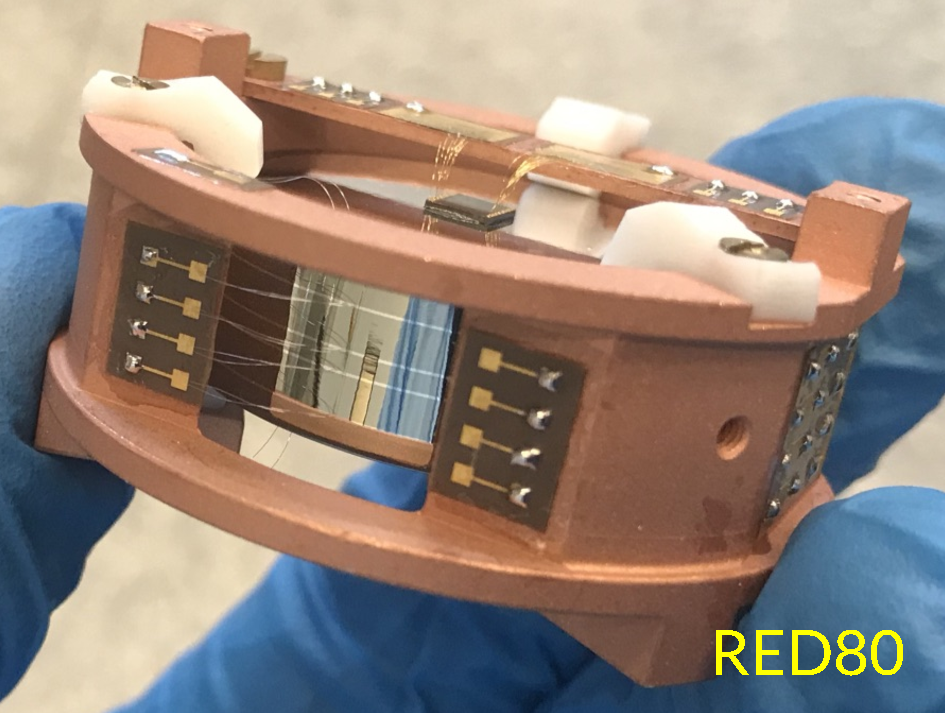
\includegraphics[align=c, scale=0.5]{Figures/ElectrodesExperimental/photo_red80_v2.pdf}
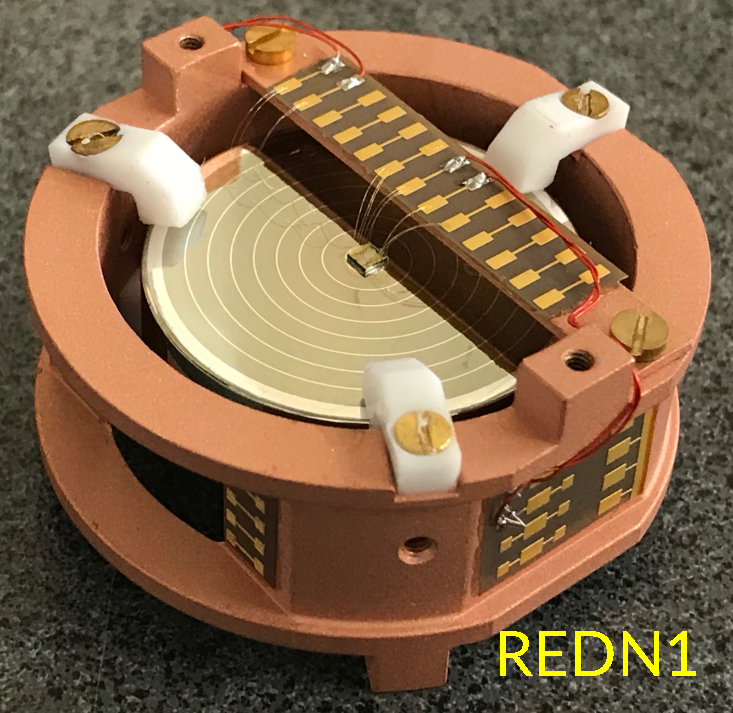
\includegraphics[align=c, scale=0.5]{Figures/ElectrodesExperimental/photo_redn1_v2.pdf}
\caption{Photos of the detector RED80 and REDN1 taken during their montage. The covers of the copper chassis are removed to finish the cabling. (Reference necessary to Stefanos ?)}
\label{fig:photo-redn1-red80}
\end{figure}

Each detector has its own particularities which are assessed in the following paragraphs \ref{par:red80-presentation} and \ref{par:redn1-presentation} dedicated to the design and the electrostatics simulation of RED80 and REDN1 respectively.


\subsection{RED80 detector}
\label{par:red80-presentation}

The description of RED80 is accompanied with the figure $\ref{fig:red80-scheme}$ displaying a cross-section scheme of the detector. This scheme is used as reference for the electrostatics simulation. The scheme is not at scale and all the dimensions used in the simulation are listed in the table \ref{tab:red80-default-parameters}.
% copper chassis
The copper chassis is modeled by an exterior electrically grounded rectangle. The germanium crystal is held is separated from the germanium crystal by vacuum represented by the light blue surrounding volume.
% teflon clamps
The Teflon clamps are not represented in the scheme and are not a part of the simulation as discussed in paragraph \ref{par:simulation-limitations}.
% heat channel
The heat channel of RED80 consists in the GeNTD thermistance labeled K58. Its dimensions are the larger Edelweiss standard of \SI{4 x 4 x 0.45}{\mm}. It is glued on aluminium at the center of the top surface as represented by the white rectangle. Although represented, the NTD is not simulated as discussed in paragraph \ref{par:simulation-limitations}.
% ionization channel
The ionization channel consists in four electrodes labeled $A$ through $D$ separated in pairs of collecting and guard electrodes. Each aluminium deposit is labeled on the scheme $\ref{fig:red80-scheme}$ according to the electrode it is attributed to.
The main electrodes are $B$ and $D$. They consists of two planar full aluminium electrodes of radius $r_{center} = \SI{13.5}{\mm}$ centered on the top and bottom surface of the germanium crystal. The role of these electrodes is to collect the majority of the drifting charges produced in the crystal. As such, they are deemed "collect electrodes".
The auxiliary electrodes are $A$ and $C$. They are formed by two pairs of circular rings of width $w_{Al}=\SI{100}{\micro\meter}$ deposited on the lateral surface of the germanium crystal. In each pair, the rings are separated by the lateral spacing $d_{lat}=\SI{2.4}{\mm}$, from their center. The two pairs are spaced by the equatorial distance $d_{eq} = \SI{1}{\mm}$, from the center of the center-most rings. The function of these electrodes is to collect any charges in the periphery of the crystal as to tag any surface recoil similarly to veto electrodes principles presented in paragraph \ref{par:veto-electrode-principle}. These electrodes are deemed "guard electrodes" as opposed to the veto ones. The difference holds in their polarization and in the direction of the electric field being the same between the collect and the guard electrodes.
% Equator offset
One should not that the guard electrodes are not centered on the equator of the crystal, represented by the finely-dashed horizontal line passing through the origin $(0,0)$ in the scheme \ref{fig:red80-scheme}. Instead, the axis of mirror symmetry for the guard electrodes is the sparsely-dashed  horizontal line passing through the coordinates $(0, z_{eq})=(0, -0.5)\si{\mm}$. This is the result of an offset in height of the mask used during the deposition of the aluminium rings. While this feature is unintentional as it induces an slight asymmetry in the design of RED80, it shall provides interesting insights considering the intrinsic asymmetry of the electron and hole drift in the semi-conducting germanium as discussed in paragraph \ref{par:charge-drift}.

\begin{figure}
\centering
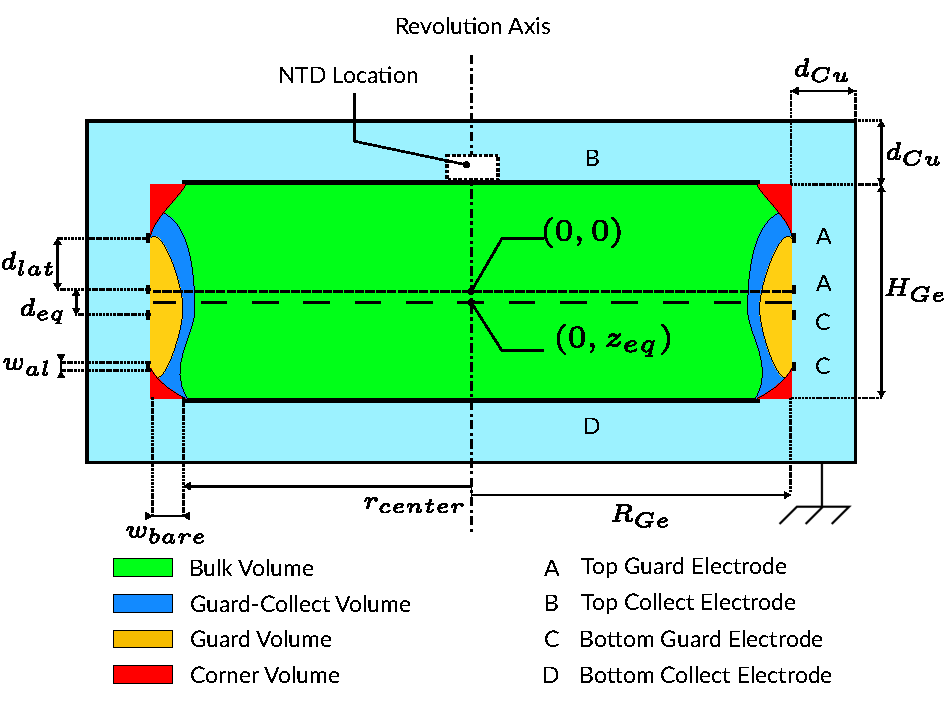
\includegraphics[scale=1]{Figures/ElectrodesExperimental/scheme_red80.pdf}
\caption{Cross-section scheme of the RED80 detector. This scheme is not at scale and the main dimensions are listed in the table \ref{tab:red80-default-parameters}. The dashed horizontal lines are axis of symmetry: finely-dashed through $(0,0)$ is for the crystal, sparsely-dashed through $(0, z_{eq})=(0, -0.5)\si{\mm}$  is for the guard rings $A,C$. The electrically grounded rectangle is the cooper chassis separated from the germanium crystal by vacuum in light blue. The aluminium pads and rings are represented in black at the surface of the crystal and labeled according to their electrode of attribution. The default potential of the electrodes are $(V_A, V_B, V_C, V_D) = (+1, +1, -1, -1) \si{\volt}$. The colored volumes inside the crystal are drawn from electric field lines with common start and end points.}
\label{fig:red80-scheme}
\end{figure}

\begin{table}[]
\centering
%\resizebox{\textwidth}{!}{%
\begin{tabular}{l c S}
Parameter                                   & Symbol        & {Default Value} \\ \hline \hline
Ge crystal Height                           & $H_{Ge}$      & \SI{10}{\mm}  \\
Ge crystal Radius                           & $R_{Ge}$      & \SI{15}{\mm}    \\
Distance between crystal and copper chassis & $d_{Cu}$      & \SI{3}{\mm}     \\
Aluminium Deposit Thickness                         & $h_{Al}$      & \SI{1}{\micro\meter}   \\
Width of the Lateral Rings                      & $w_{Al}$      & \SI{80}{\micro\meter}  \\
Radius of the Planar Electrode Pad  & $r_{center}$   & \SI{13.5}{\mm}   \\
Width of bare Ge crystal on edge     & $w_{bare}$    & \SI{1.5}{\mm}  \\
Spacing between Lateral Rings          & $d_{lat}$  & \SI{2.4}{\mm}  \\
Equatorial distance						& $d_{eq}$	& \SI{1.2}{\mm} \\
Offset on Equator Height				& $z_{eq}$	& \SI{-0.5}{\mm} \\
Main Voltage Bias                           & $V_{bias}$    & \SI{2}{\volt}      \\
Symmetric factor of the voltage bias        & $S_{bias}$    & {$0.5$}         
\end{tabular}
%}%
\caption{Parameter values for the design and default polarization of RED80.}
\label{tab:red80-default-parameters}
\end{table}

% Capacitance
The electrostatic simulation of the presented geometry yields the capacitance matrices  of the detector RED80. The convention regarding indexes introduced in the chapter \ref{ChapterElectrodes} is still in use. Each electrode is attributed to an index such that:
\begin{equation}
\label{eq:indexes-convention}
\{ A, B, C, D \} \Leftrightarrow \{ 1, 2, 3, 4 \}
\end{equation}
In this light, the Maxwell capacitance matrix associated with the electrodes of RED80 is evaluated to:
\begin{equation}
\label{eq:redn1-maxwell}
\bm{C} = 
\begin{pmatrix}
  13.93 & -6.32 & -3.89 & -2.57\\
  -6.32 & 17.17 & -1.91 & -6.06\\
  -3.89 & -1.91 & 14.25 & -7.28\\
  -2.57 & -6.06 & -7.28 & 18.61\\
\end{pmatrix}
\times \SI{e-12}{\farad}
\end{equation}
Using the equations \ref{eq:maxwell-to-mutual}, the mutual capacitance matrix of RED80 is evaluated to:
\begin{equation}
\label{eq:redn1-mutual}
\bm{C}^m = 
\begin{pmatrix}
  1.15 & 6.32 & 3.89 & 2.57\\
  6.32 & 2.88 & 1.91 & 6.06\\
  3.89 & 1.91 & 1.17 & 7.28\\
  2.57 & 6.06 & 7.28 & 2.70\\
\end{pmatrix}
\times \SI{e-12}{\farad}
\end{equation}
One remarkable property of these capacitance matrix relative to RED80, compared to the other capacitance matrices of PL38, FID38 and REDN1 discussed in this work, is the absence of symmetry between top and bottom. This is a direct consequence of the asymmetrical geometry of RED80 with its offset guard electrodes.  
According the diagonal terms of the Maxwell matrix $C_{XX}$, the main collect electrode $B,D$ displays globally more capacitive coupling than the auxiliary guard electrode $A,C$. This can be readily explained by the difference in area between the collect and guard electrodes. This interpretation is supported by the relatively high mutual capacitance term $C_{BD}^m$ associated to the opposite-sided collect electrodes $B$ and $D$. 
The coupling terms between same-sided collect and veto electrodes $C_{AB}^m$ and  $C_{CD}^m$ are the highest terms of the mutual matrix $\bm{C}^m$. This is due to the proximity of same-sided electrode. This is confirmed by the observation that $C_{CD}^m > C_{AB}^m$: the height offset $z_{eq}$ of the guard electrodes leads to a shorter 
distance between $C$ and $D$ than between $A$ and $B$.
As what was observed for in the chapter \ref{ChapterElectrodesScan} for the design PL38 and FID38, the self-capacitance terms $C_{XX}^m$ are among the smallest terms in the capacitance matrix $\bm{C}^m$. This is attributed to the high difference in relative dielectric permittivity between the germanium and the vacuum.

% Total weighting potential
Without fixing the polarization of RED80 yet, the electrostatics can yield the map of the total weighting potential presented in the figure \ref{fig:red80-potential-twp}.  As discussed in \ref{ref:shockley-ramo}, the Shockley-Ramo theorem indicates that this total weighting potential indicates the quality of the Faraday cage formed by the RED80 electrodes, which is of paramount importance for trapped charges which does not reach the electrodes.
The corners display a lessened total weighting potential due to the absence of aluminium deposit in these regions.

% Polarization
For standard operation, same-sided guard and collect electrodes have the same electric potential. The polarization of the detector can therefore be fixed with two parameters such that:
\begin{align}
V_A = V_B = & V_{bias} \cdot S_{bias} \\
V_C = V_D = & - V_{bias} \cdot \left( 1 - S_{bias} \right)
\end{align}
with $V_{bias}$ being the bias voltage and $S_{bias}$ the polarization symmetry parameter.
The default polarization is set at $\left( V_{bias}, S_{bias} \right) = (\SI{2}{\volt}, 0.5)$. In this state, the electric potential of the electrodes are:
\begin{equation}
(V_A, V_B, V_C, V_D) = (+1, +1, -1, -1)\ \si{\volt}
\end{equation}

% Potential and E field
With this polarization, the electrostatic equations are numerically solved. The figure \ref{fig:red80-potential-twp} presents a map of the electric potential with isopotential contours. The  figure \ref{fig:red80-efield} displays two graph relative to the electric field. On the left is the map of the magnitude of the electric field $\| \bm{E} \|$ with a white overlay representing the electric field lines. On the right is the histogram and the cumulative distribution function of the magnitude distribution over the crystal volume.
Apart from the periphery of the crystal, the volume of RED80 hosts neatly equally spaced isopotential contours. As a result, the electric field norm is indeed uniform in the crystal and the field lines are all parallel and vertical linking the collect electrodes $B$ and $D$. Indeed, the magnitude distribution features a neatly define peak at $\| \bm{E} \| = \SI{2}{\volt\per\centi\meter}$.
Near the lateral surface, the field lines now link the guard electrodes and collect electrodes. The equatorial region has high electric field norm due to the close equatorial guard rings. This participates at broadening the magnitude distribution towards value greater than the median \SI{2}{\volt\per\centi\meter}.
On the contrary, the corners show very low magnitude values which coincide with divergence points for the electric field lines. It seems like in the corners of the crystal, the field lines leave the crystal to end on the copper chassis. This observation observation leads us to expect surface trapping in the corners. It also explains the electric field magnitude extension at lowest value .

% Fiducial Volume
An advanced study of the field lines can separate the crystal volume in several regions with different collecting behavior depending on the start and the end point of the field lines. For RED80, there are four different regions which are drawn on the scheme \ref{fig:red80-scheme}. 
The main region is the "bulk volume" also called "fiducial volume", colored in green on the scheme, and corresponds to field lines linking the two main collect electrodes $B$ ad $D$. Its volume is the important theoretical fiducial volume. At default polarization, its percentage is estimated at $\%_{fid}=\SI{80.75}{\percent}$. This value is obtained with the method discussed in paragraph \ref{par:fiducial-volume}. The percentage of the volume attributed to other regions is less precise due to the limitation of the estimation technique.
On the lateral surface of the crystal, the electric field lines linking the two guard electrodes $A$ and $C$ form the so-called "guard volume" illustrated as the orange region on the scheme. Its volume percentage is estimated to $\%_{guard} \approx \SI{7}{\percent}$. 
As a consequence of the height offset $z_{eq}$ of the guard electrodes, a significant portion of the electric field lines start on the top guard electrode $A$ and end on the bottom collect electrode $D$. These lines draw the blue region deemed "guard-collect volume". Its volume percentage is approximated to $\%_{guard-collect} \approx \SI{6}{\percent}$.
The last volume corresponds to the corner regions with the field lines leaving the crystal to end on the cooper chassis. This so-called "corner volume" is colored red and has a volume percentage of about $\%_{corners} \approx \SI{5}{\percent}$.

Each region has a specific electric charge signal vector $\vec{Q}$ induced by a number $N_p$ of electron-hole pairs created in the crystal such that $Q = N_p e$. Assuming an ideal charge collection following the electric field lines and without transversal component, the Shockley-Ramo is used to express the first three charge vectors:
\begin{equation}
\label{eq:red80-induced-charges}
\vec{Q}_{bulk} =
\begin{bmatrix}
0 \\ -1 \\ 0 \\ 1
\end{bmatrix}
\cdot N_p \cdot e
\quad ; \quad
\vec{Q}_{guard} =
\begin{bmatrix}
-1 \\ 0 \\ 1 \\ 0
\end{bmatrix}
\cdot N_p \cdot e
\quad ; \quad
\vec{Q}_{guard-collect} =
\begin{bmatrix}
-1 \\ 0 \\ 0 \\ 1
\end{bmatrix}
\cdot N_p \cdot e
\end{equation}

The charge vector corresponding to the corner volume $Q_{corner}$ is not readily available as all the drifting charge should theoretically be subject to surface trapping.

\begin{figure}
\centering
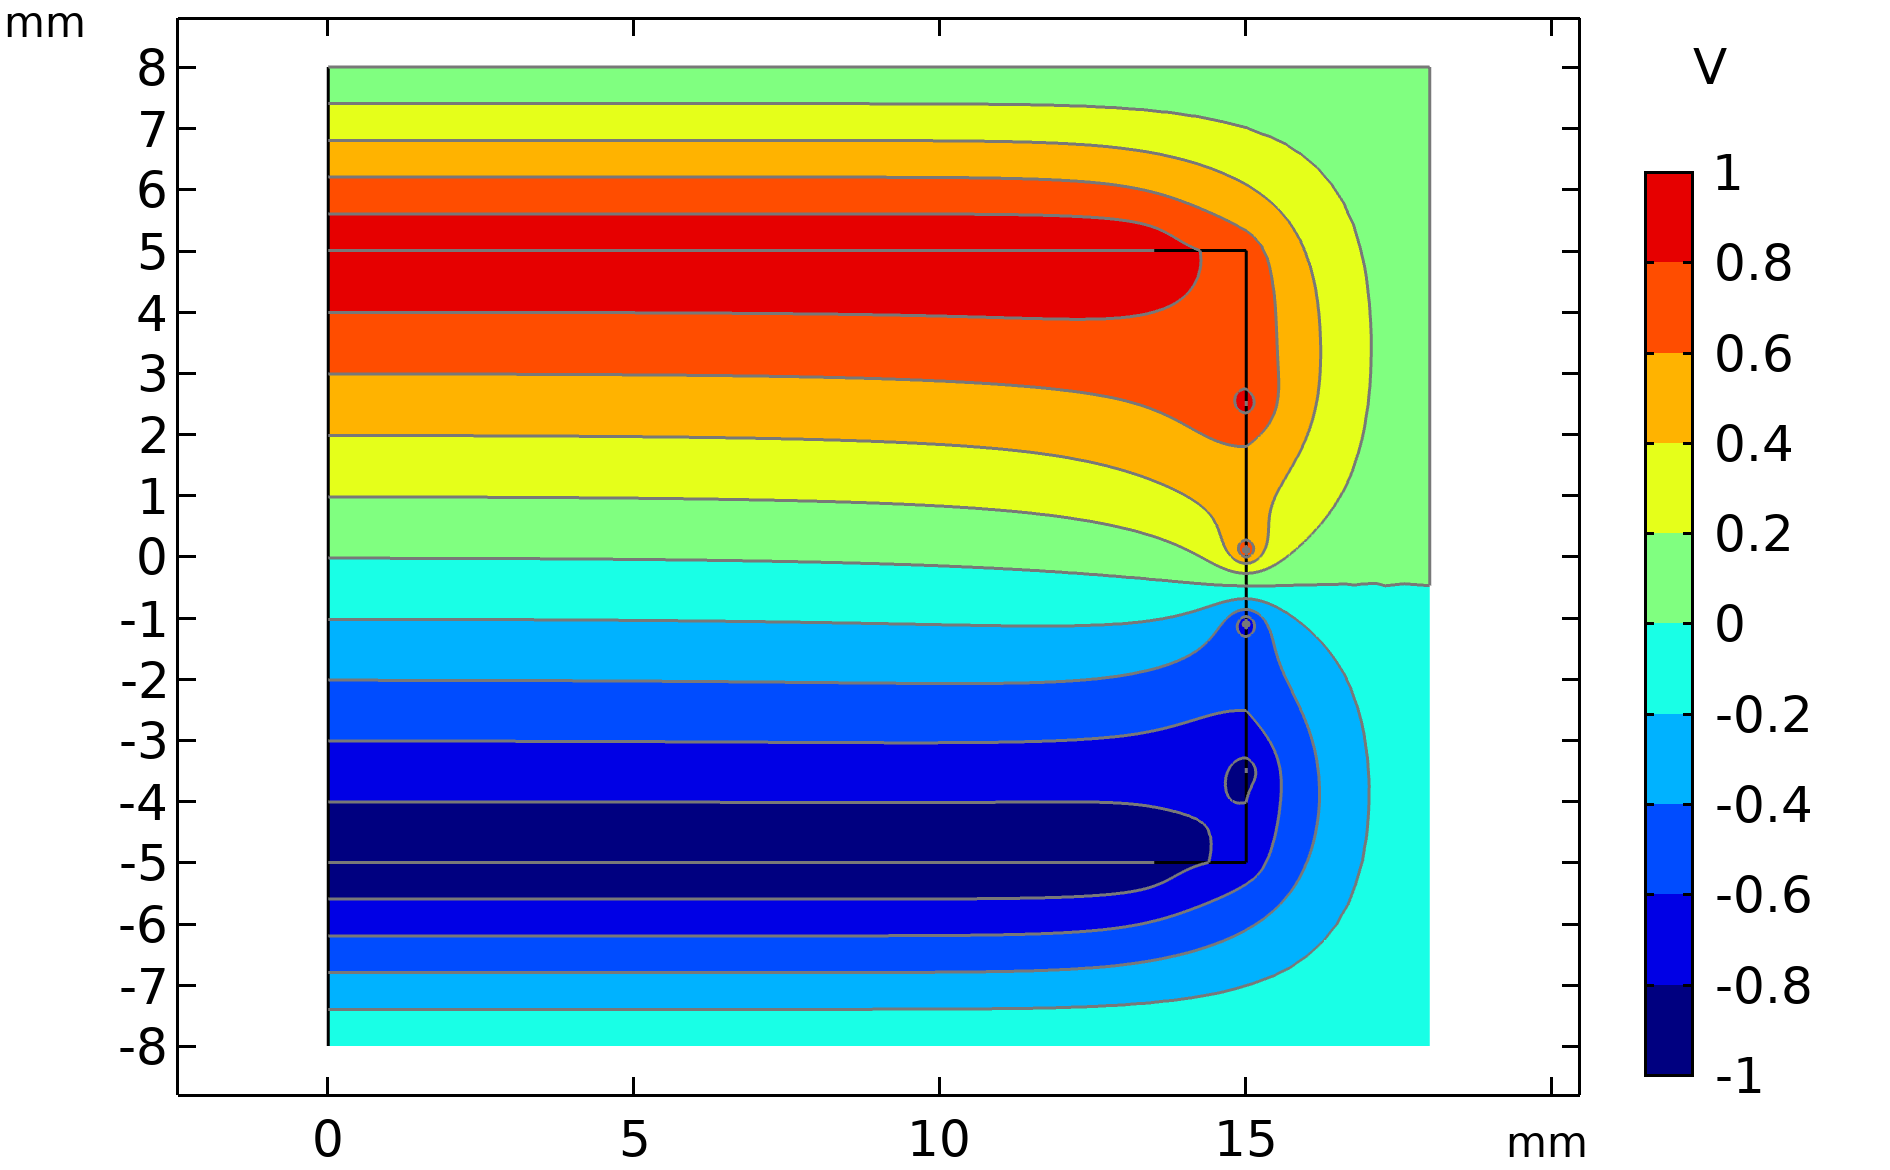
\includegraphics[scale=0.5]{Figures/ElectrodesExperimental/potential_red80.png}
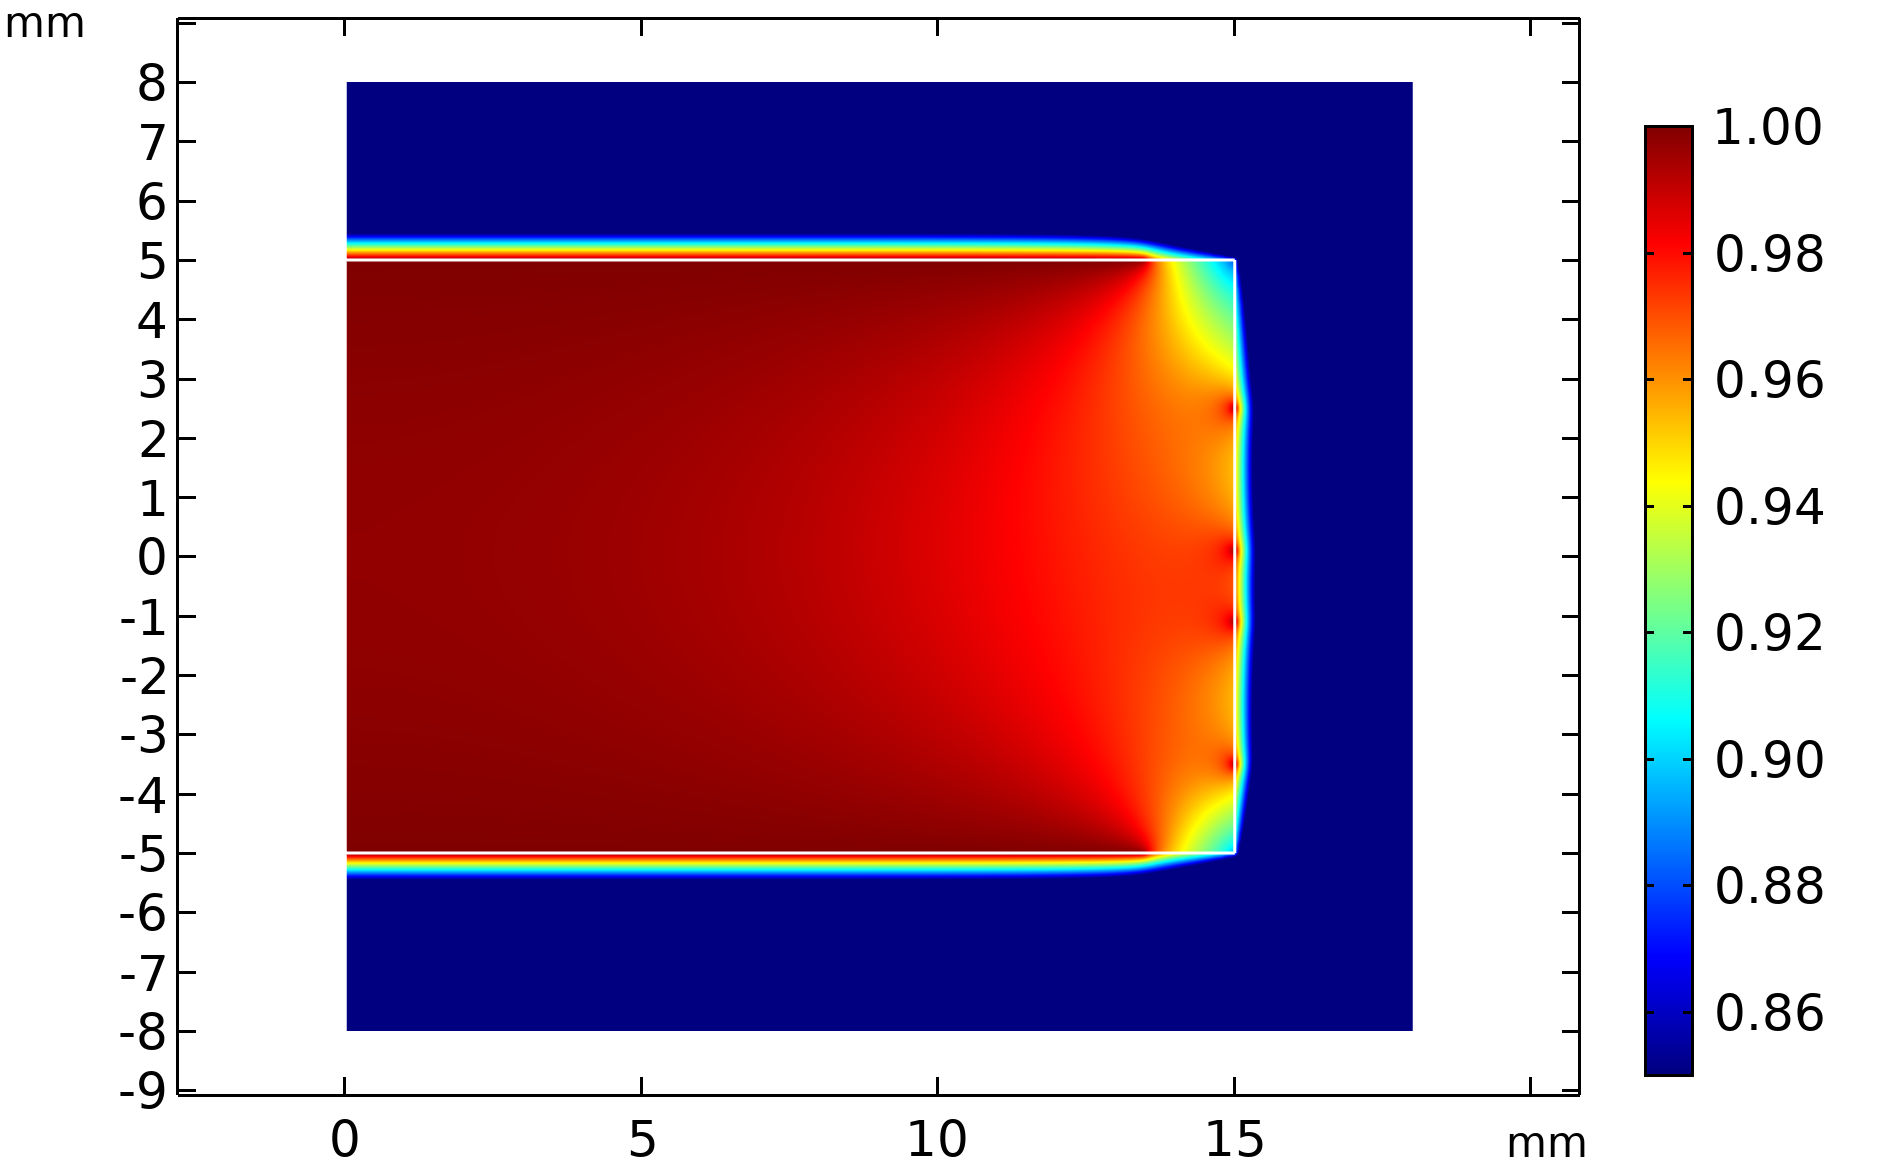
\includegraphics[scale=0.5]{Figures/ElectrodesExperimental/twp_red80.png}
\caption{Color maps of the electric potential (on the left) and the total weighting potential (on the right) from the simulation of RED80. For the left graph, the default polarization is used.}
\label{fig:red80-potential-twp}
\end{figure}

\begin{figure}
\centering
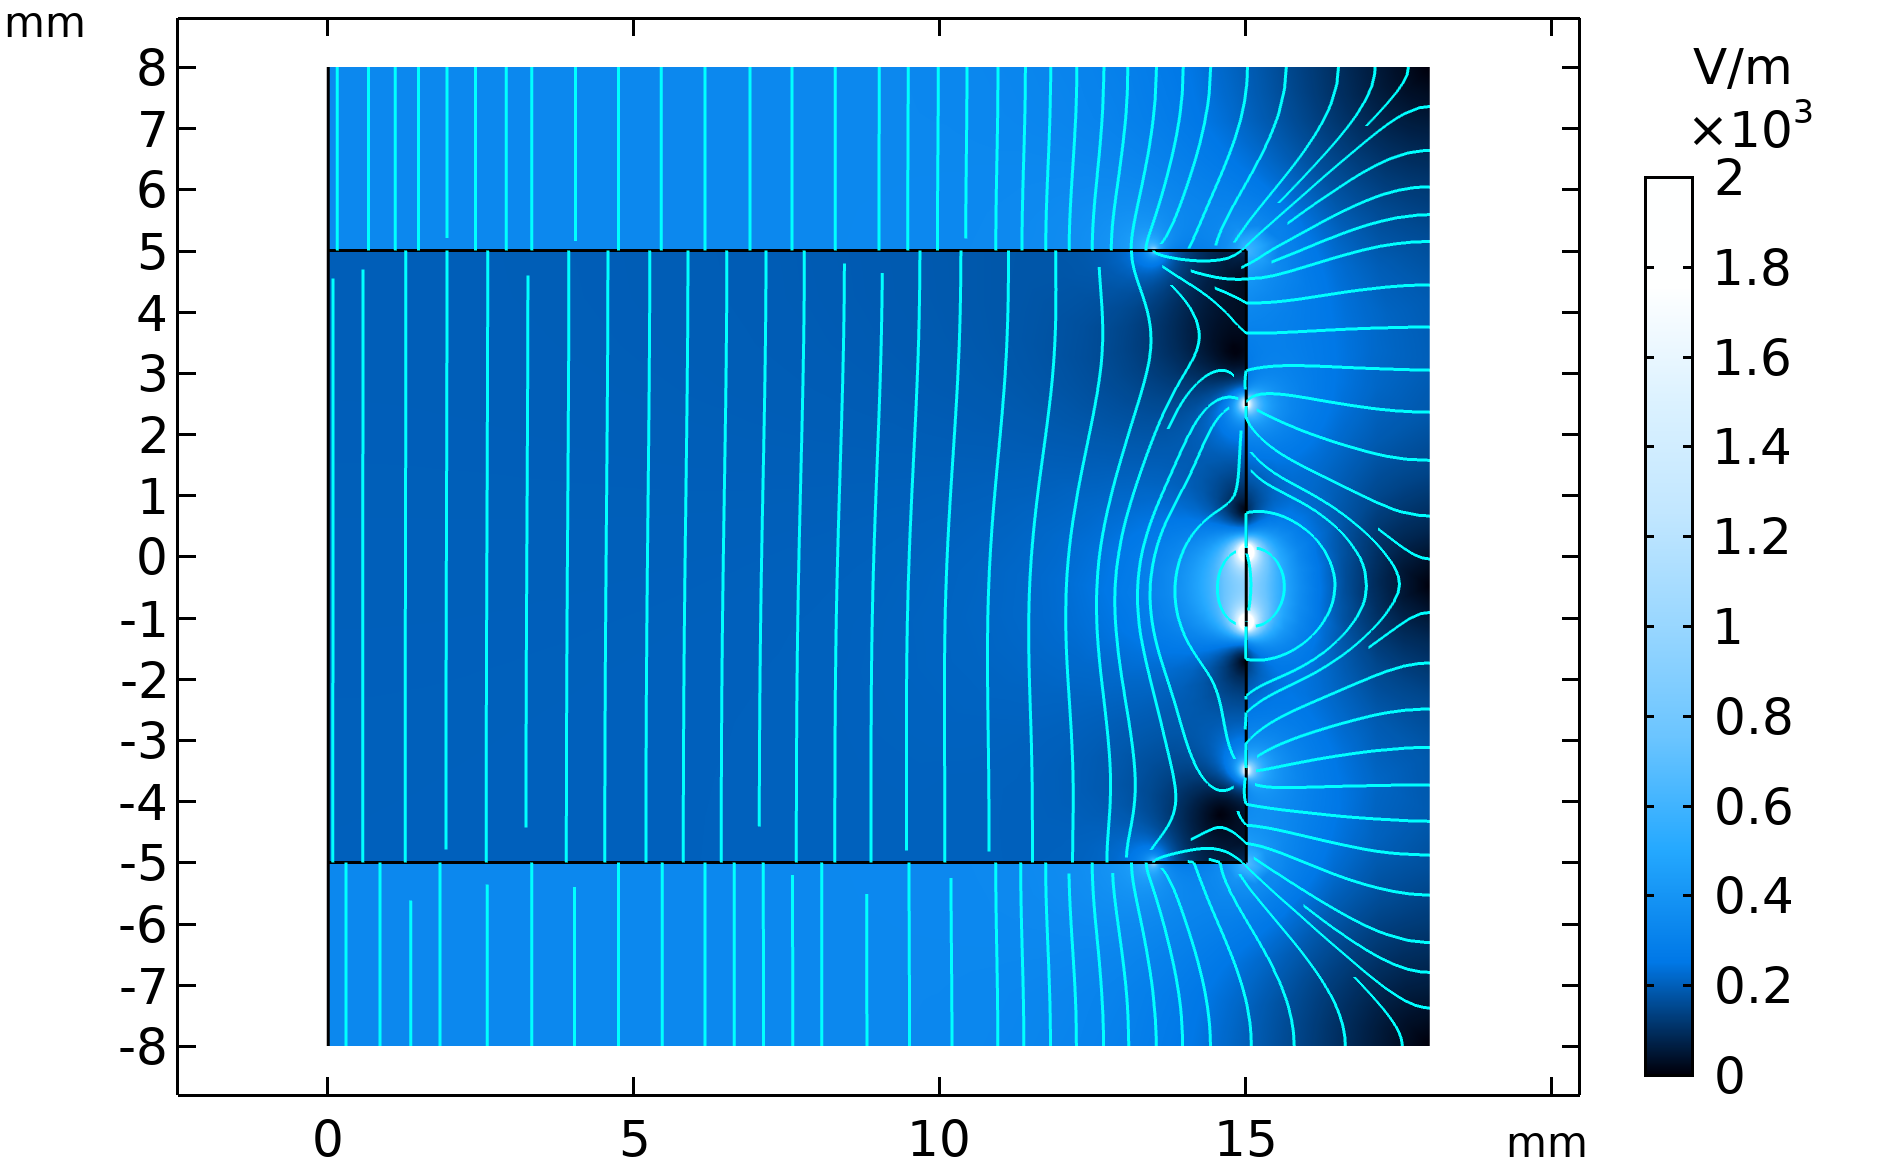
\includegraphics[align=c, scale=0.5]{Figures/ElectrodesExperimental/efield_red80.png}
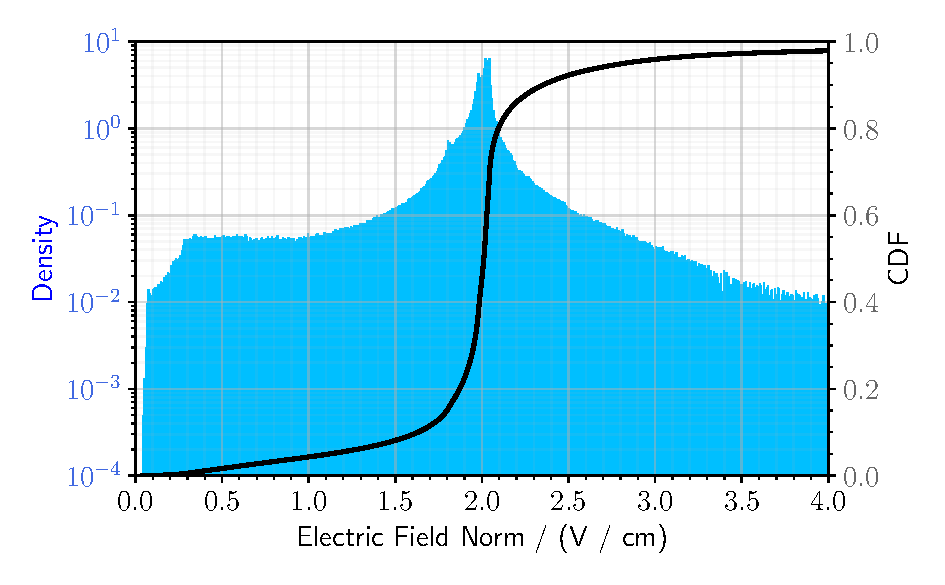
\includegraphics[align=c, scale=0.5]{Figures/ElectrodesExperimental/enorm_hist_red80.pdf}
\caption{(On the left) Color map of the magnitude of the electric field with white representation of the electric field lines from the simulation of RED80. The default polarization is used. The colored volumes in the scheme \ref{fig:red80-scheme} are drawn from the electric field lines with common start and end points.
(On the right) Histogram and Cumulative Distribution Function of the distribution of the magnitude of the electric field over the crystal volume from the simulation of RED80.}
\label{fig:red80-efield}
\end{figure}

In the later paragraph \ref{par:red80-comparison}, the RED80 simulation presented here is compared to the experimental data taken during the operation of RED80. In particular, a scan over the voltage bias $V_{bias}$ is performed. As discussed in the previous chapter \ref{ChapterElectrodesScan} with the scans of the designs PL38 and FID38, a change of the voltage bias solely scale the magnitude of the electric field in the crystal. Any other quantities deduced from the simulation of RED80, like the fiducial volume and the capacitance matrices, are unaffected.


\subsection{REDN1 detector}
\label{par:redn1-presentation}

The description of REDN1 is illustrated with the figure \ref{fig:redn1-scheme} displaying a cross-section scheme of the detector. This scheme is used as reference for the electrostatics simulation. The scheme is not at scale and all the dimensions used in the simulation are listed in the table \ref{tab:redn1-default-parameters}.
% copper chassis
The copper chassis is modeled by an exterior electrically grounded rectangle. The germanium crystal is held is separated from the germanium crystal by vacuum represented by the light blue surrounding volume.
% teflon clamps
The Teflon clamps are not represented in the scheme and are not a part of the simulation as discussed in paragraph \ref{par:simulation-limitations}.
% heat channel
The heat channel of REDN1 consists in a NTD of small standard dimensions \SI{2 x 2 x 0.45}{\mm}. It is glued on aluminium at the center of the top surface as represented by the white rectangle. Although represented, the NTD is not simulated as discussed in paragraph \ref{par:simulation-limitations}.
% ionization channel
The ionization channel of REDN1 has an electrode geometry called Inter Digitized (ID) differing from the FID geometry by not having any aluminium deposit on the lateral surface. Each electrodes is composed of multiples aluminium rings or pads linked with aluminium-wire bridge. There is a central pad of radius $r_{center}=\SI{1.5}{\mm}$ on the top and bottom planar surface of the crystal. The top central pad hosts the NTD thermal sensor. Surrounding the central pads are $7$ thin concentric rings of width $w_{Al} = \SI{80}{\micro\meter}$. The crystal edges features large outer rings of width $w_{outer}=\SI{1}{\mm}$. As a result, each planar surface possesses a number $n_{plan}=9$ of distinct aluminium deposits. Each deposit, ring and pad, are centered and distanced from their neighbor by the planar spacing $d_{plan} = \SI{1.563}{\mm}$.
% electrode attribution
The ionization channel of REDN1 consists in four electrodes labeled $A$ through $D$. The aluminium deposits of the top (resp. bottom) surface are attributed to the electrodes $A,B$ (resp. $C,D$) according the labels on the scheme \ref{fig:redn1-scheme}.
The main electrodes are $B$ and $D$. Their function is to collect the drifting charges produced in the bulk of the crystal. As such, they are deemed "collect electrodes".
The auxiliary electrodes are $A$ and $C$. Their role is to collect any charges produced near the surface of the crystal. As for the FID detectors, these electrodes allow for the tagging of any surface recoil as explained in paragraph \ref{par:veto-electrode-principle}. The denomination "veto electrodes" is kept for these electrodes.
Same-sided collect and veto electrodes have their aluminium rings interleaved as to correctly shape the electric field. As to correlate tag recoil happening on the lateral surface and under the NTD, the central pads and the outermost large rings are attributed to the veto electrodes $A$ and $C$. 

\begin{table}[]
\centering
%\resizebox{\textwidth}{!}{%
\begin{tabular}{l c S}
Parameter                                   & Symbol        & {Default Value} \\ \hline \hline
Ge crystal Height                           & $H_{Ge}$      & \SI{10}{\mm}  \\
Ge crystal Radius                           & $R_{Ge}$      & \SI{15}{\mm}    \\
Distance between crystal and copper chassis & $d_{Cu}$      & \SI{3}{\mm}     \\
Electrode Thickness                         & $h_{Al}$      & \SI{1}{\micro\meter}   \\
Electrode Width                             & $w_{Al}$      & \SI{100}{\micro\meter}  \\
Radius of the innermost planar electrode    & $r_{center}$   & \SI{1.5}{\mm}   \\
Width of bare Ge crystal on corners      & $w_{bare}$    & \SI{0}{\mm}  \\
Width of the outermost veto electrode    & $w_{outer}$    & \SI{1}{\mm}  \\
Number of planar electrodes                 & $n_{plan}$  & {$9$}             \\
Interdistance of Planar electrodes          & $d_{plan}$  & \SI{1.563}{\mm}  \\
Main Voltage Bias                           & $V_{bias}$    & \SI{2}{\volt}      \\
Ratio Veto/Main voltage bias                & $R_{veto}$    & {$0.4$}         \\
Symmetric factor of the voltage bias        & $S_{bias}$    & {$0.5$}         
\end{tabular}
%}%
\caption{Parameter values for the design and default polarization of REDN1.}
\label{tab:redn1-default-parameters}
\end{table}

\begin{figure}
\centering
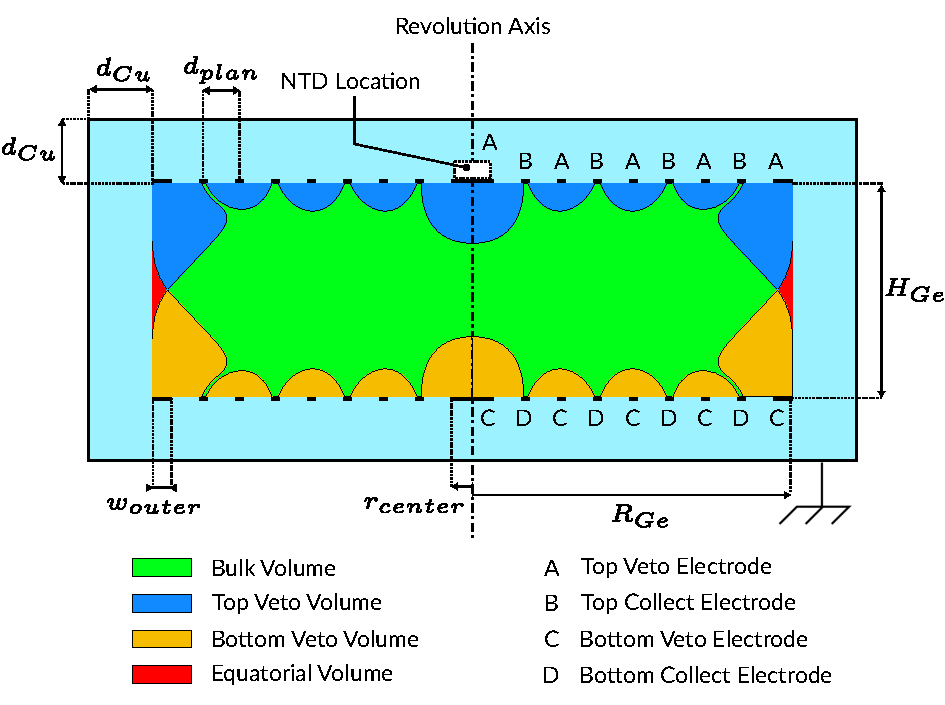
\includegraphics[scale=1]{Figures/ElectrodesExperimental/scheme_redn1.pdf}
\caption{Cross-section scheme of the REDN1 detector. This scheme is not at scale and the main dimensions are listed in the table \ref{tab:redn1-default-parameters}. The electrically grounded rectangle is the cooper chassis separated from the germanium crystal by vacuum in light blue. The aluminium pads and rings are represented in black at the surface of the crystal and labeled according to their electrode of attribution. The default potential of the electrodes are $(V_A, V_B, V_C, V_D) = (-0.4, +1, +0.4, -1) \si{\volt}$. The colored volumes inside the crystal are drawn from electric field lines with common start and end points.}
\label{fig:redn1-scheme}
\end{figure}

% Capacitance
With the now fixed electrode geometry, the electrostatics simulation is run and can output the capacitance matrices relative to REDN1. The usual equivalence between electrodes and indexes displayed in equation \ref{eq:indexes-convention} is in use. As such, the Maxwell capacitance matrix associated with the electrodes of REDN1 is evaluated to:
\begin{equation}
\label{eq:redn1-maxwell}
\bm{C} = 
\begin{pmatrix}
  19.46 & -11.84 & -3.00 & -1.89\\
  -11.84 & 16.17 & -1.89 & -1.26\\
  -3.00 & -1.89 & 19.46 & -11.84\\
  -1.89 & -1.26 & -11.84 & 16.17\\
\end{pmatrix}
\times \SI{e-12}{\farad}
\end{equation}
Using the equations \ref{eq:maxwell-to-mutual}, the mutual capacitance matrix of REDN1 is evaluated to:
\begin{equation}
\label{eq:redn1-mutual}
\bm{C}^m = 
\begin{pmatrix}
  2.73 & 11.84 & 3.00 & 1.89\\
  11.84 & 1.18 & 1.89 & 1.26\\
  3.00 & 1.89 & 2.73 & 11.84\\
  1.89 & 1.26 & 11.84 & 1.18\\
\end{pmatrix}
\times \SI{e-12}{\farad}
\end{equation}
The hierarchy of the capacitance terms of REDN1 is very similar to the one discussed for the design FID38 in paragraph \ref{par:fid38-capacitance}. The dominant capacitance terms are the one associated to same-sided collect and veto electrodes $C_{AB}^m=C_{CD}$. This is explained by same-sided electrodes having interleaved rings thus emulating a high area and low distance in regards to their capacitive coupling.
As usual, the self-capacitance $c_{XX}^m$ are small due to the high dielectric constant of the germanium compared to vacuum.
The only significant difference between REDN1 and FID38 is the relatively low capacitance term between the veto electrodes $C_{AC}^m$ in the case of REDN1. Indeed, as this detector has no aluminium deposit on its lateral surface, it does not have the equatorial veto rings notorious for their low equatorial distance $d_{eq}$ leading to heightened capacitance. 

% Total weighting potential
Another result independent from the polarization of REDN1 is the map of the total weighting potential presented in the figure \ref{fig:redn1-potential-twp}.  As discussed in \ref{ref:shockley-ramo}, the Shockley-Ramo theorem indicates that this total weighting potential indicates the quality of the Faraday cage formed by the REDN1 electrodes, which is of paramount importance for trapped charges which does not reach the electrodes. 
In this graph, red colored regions corresponds to a total weighting potential tending to the unity, thus mitigating the adverse effect of charge trapping on the signal generation. These regions are mostly presents near the electrodes and near the center of the crystal. 
Blue-colored regions indicates a lower total weighting potential and are present on the periphery of the crystal. This is due to the absence of aluminium deposit on the lateral surface of REDN1. As such, a significant portion of the signal is induced on the grounded chassis.
%We can expect significant loss in signal is lateral surface is expected to be prone to surface trapping

% Polarization
The polarization of REDN1 is the same as the design FID38 which is displayed in equation \ref{eq:fid-polarization}. The potential of the electrodes are fixed by the same three parameters the bias voltage $V_{bias}$, the polarization symmetry $S_{bias}$ and the polarization ratio $R_{veto}$.
The default polarization is set at $\left( V_{bias}, S_{bias}, R_{veto} \right) = (\SI{2}{\volt}, 0.5, 0.4)$. In this state, the electric potential of the electrodes are:
\begin{equation}
(V_A, V_B, V_C, V_D) = (-0.4, +1, +0.4, -1)\ \si{\volt}
\end{equation}

% Potential and E field
The electrostatic equations are numerically solved using this default polarization. The figure \ref{fig:redn1-potential-twp} presents a map of the electric potential with isopotential contours. The  figure \ref{fig:redn1-efield} displays two graph relative to the electric field. On the left is the map of the magnitude of the electric field $\| \bm{E} \|$ with a white overlay representing the electric field lines. On the right is the histogram and the cumulative distribution function of the magnitude distribution over the crystal volume.
Apart from the periphery of the crystal, the electric potential and magnitude are very similar of the ones obtained with the simulation of the FID38 design. In the bulk of the crystal, the electric field is almost uniform and participates to the magnitude peak at $\| \bm{E} \| = \SI{0.4}{\volt\per\centi\meter}$. 
On the top and bottom surface, the alternating potential volume shape the electric field line to form veto volumes. As the electric field is nullified under the veto rings, we observe associated small low magnitude regions. As for the veto central pads, they induces an apparently larger central low magnitude region whose volume is low as it does not benefit from the rotation.
The electric field on the lateral surface of the crystal is dominated by the influence of the large outermost veto rings and the grounded chassis. The electric field is nullified close to equator at the divergence point for the field lines.
The CDF of the magnitude distribution conform that a significant fraction of the volume has a low magnitude value.

% Fiducial Volume
A close study of the field lines separates the crystal volume in several regions with different collecting behavior depending on the start and the end point of the field lines. For REDN1, there are four different regions which are drawn on the scheme \ref{fig:redn1-scheme}. 
The main region is the "bulk volume" also called "fiducial volume", colored in green on the scheme, and corresponds to field lines linking the two main collect electrodes $B$ ad $D$. Its volume is the important theoretical fiducial volume. At default polarization, its percentage is estimated at $\%_{fid}=\SI{51.75}{\percent}$.
Near the top (resp. bottom) surface of the crystal, the electric field lines link the same-sided veto and collect electrodes $A$ and $B$ (resp. $C$ and $D$). Just as for the FID38 design, this regions is called the top (resp. bottom) veto volume and is colored in blue (resp. orange) on the scheme. The estimated theoretical volume percentages of the top or bottom veto volumes are $\%_{top,veto} = \%_{bottom,veto} \approx \SI{22}{\percent}$. 
The last volume is drawn by the field lines connecting the top and bottom veto electrodes $A$ and $C$, even though a majority of these field lines leave the crystal. The denomination "equatorial volume" is in use and it is illustrated by the red region near the equator. Its volume percentage is of about $\%_{equator} \approx \SI{2}{\percent}$.

% Charge vectors
Each region has a specific electric charge signal vector $\vec{Q}$ induced by a number $N_p$ of electron-hole pairs created in the crystal such that $Q = N_p e$. We consider an ideal charge collection where electron and hole trajectories corresponds to the field lines. The charge vectors are the same as for the design FID38 displayed in equation \ref{eq:fig38-charge-vectors}.
Assuming the electric charges exactly follows the electric field lines, the overwhelming majority of the charges produced in the equatorial volume should be trapped on the lateral surface of the crystal. As such, the charge vector $\vec{Q}_{equator}$ would depends on the weighting potential of each electrodes on the lateral surface.

\begin{figure}
\centering
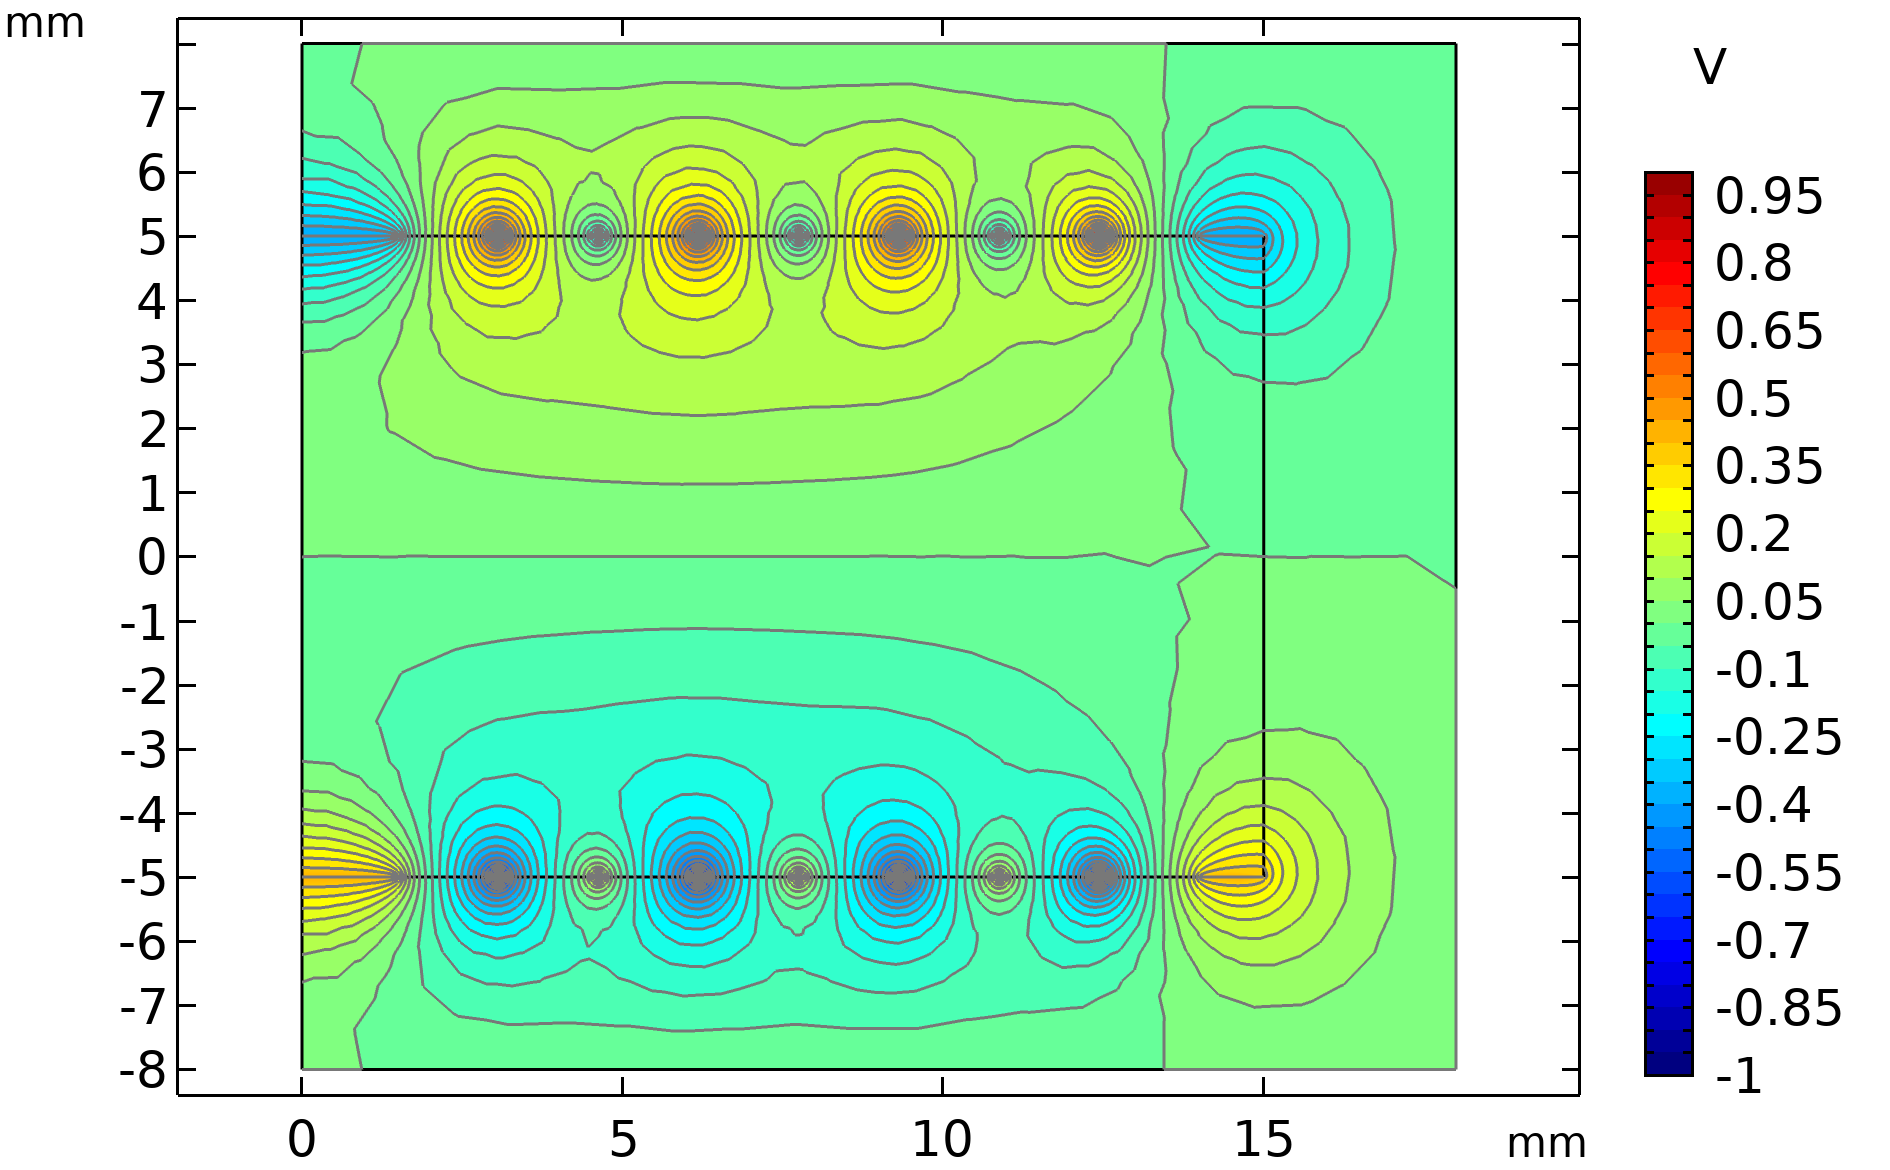
\includegraphics[scale=0.5]{Figures/ElectrodesExperimental/potential_redn1.png}
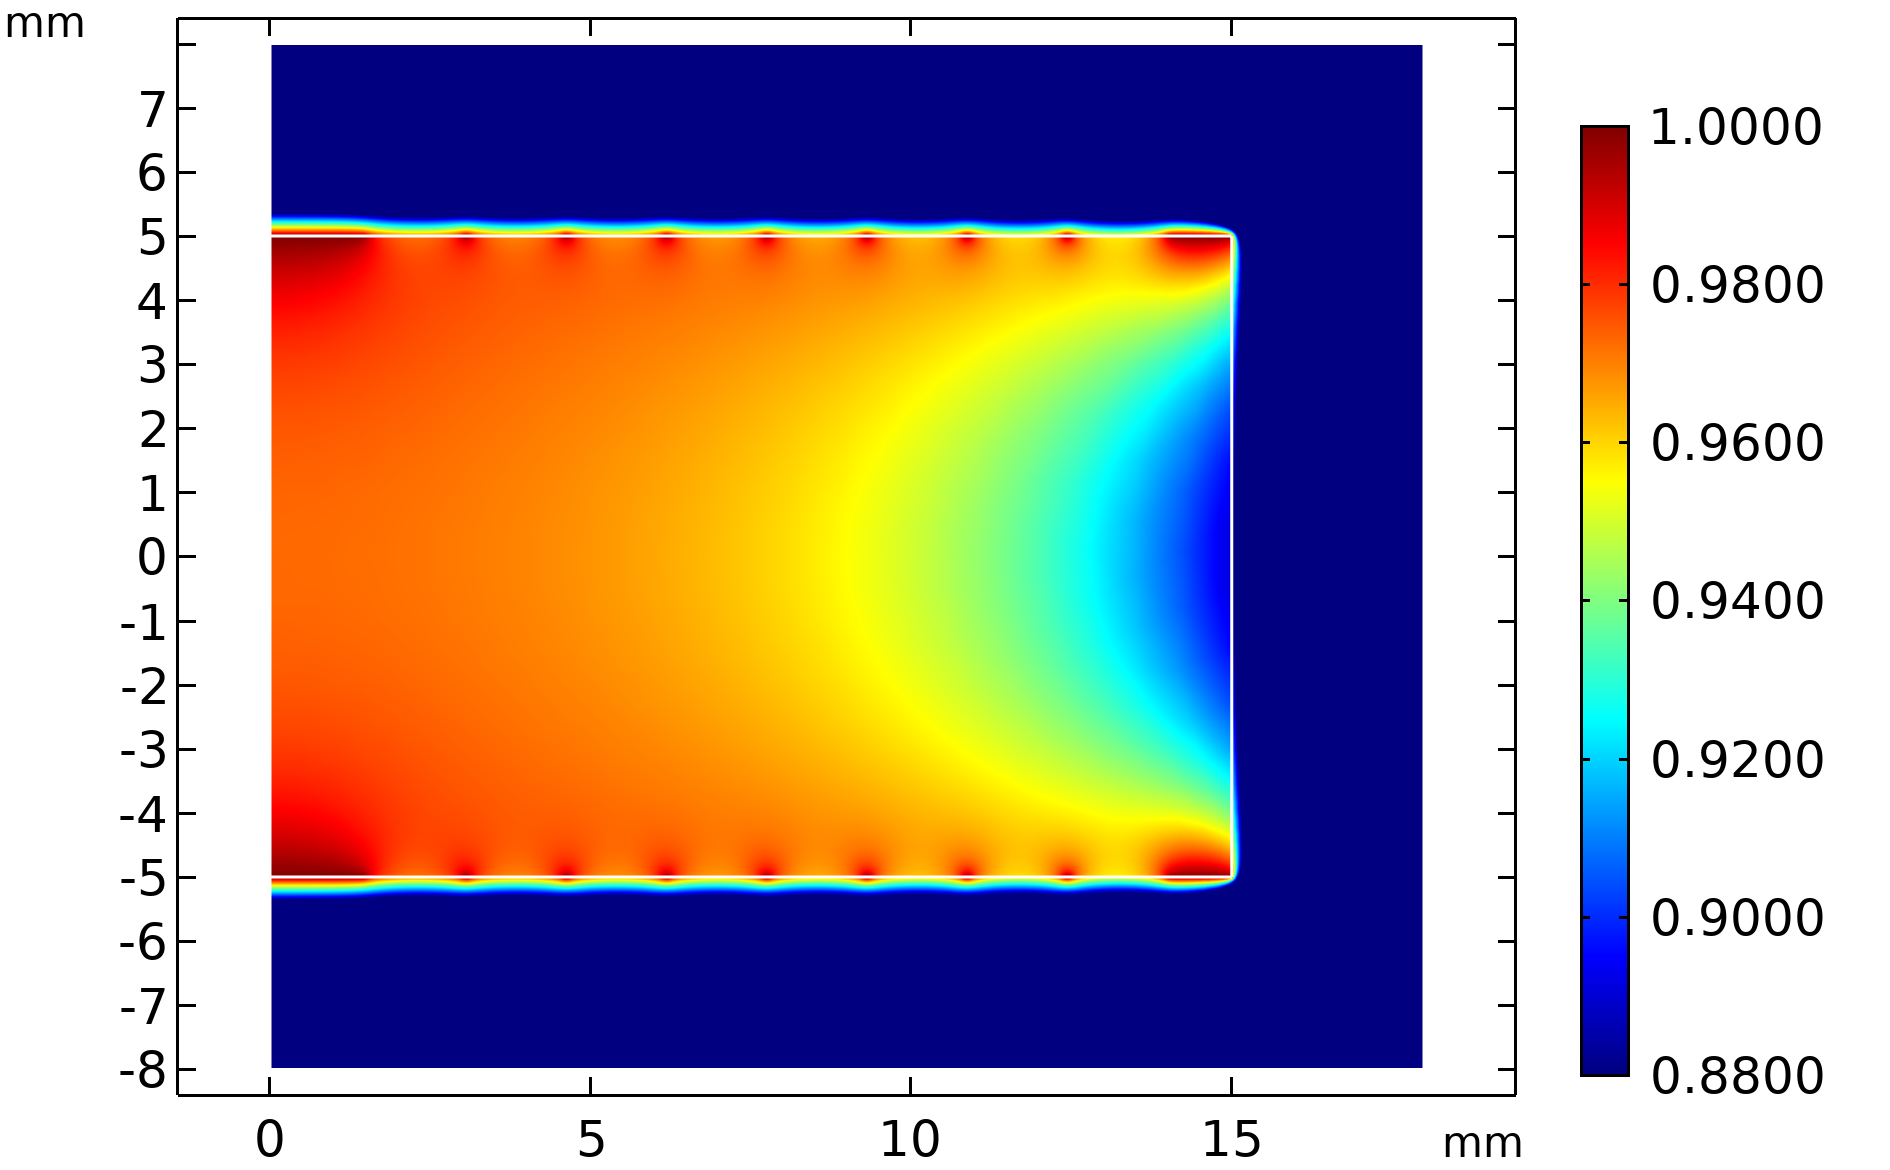
\includegraphics[scale=0.5]{Figures/ElectrodesExperimental/twp_redn1.png}
\caption{Color maps of the electric potential (on the left) and the total weighting potential (on the right) from the simulation of REDN1. For the left graph, the default polarization is used.}
\label{fig:redn1-potential-twp}
\end{figure}

\begin{figure}
\centering
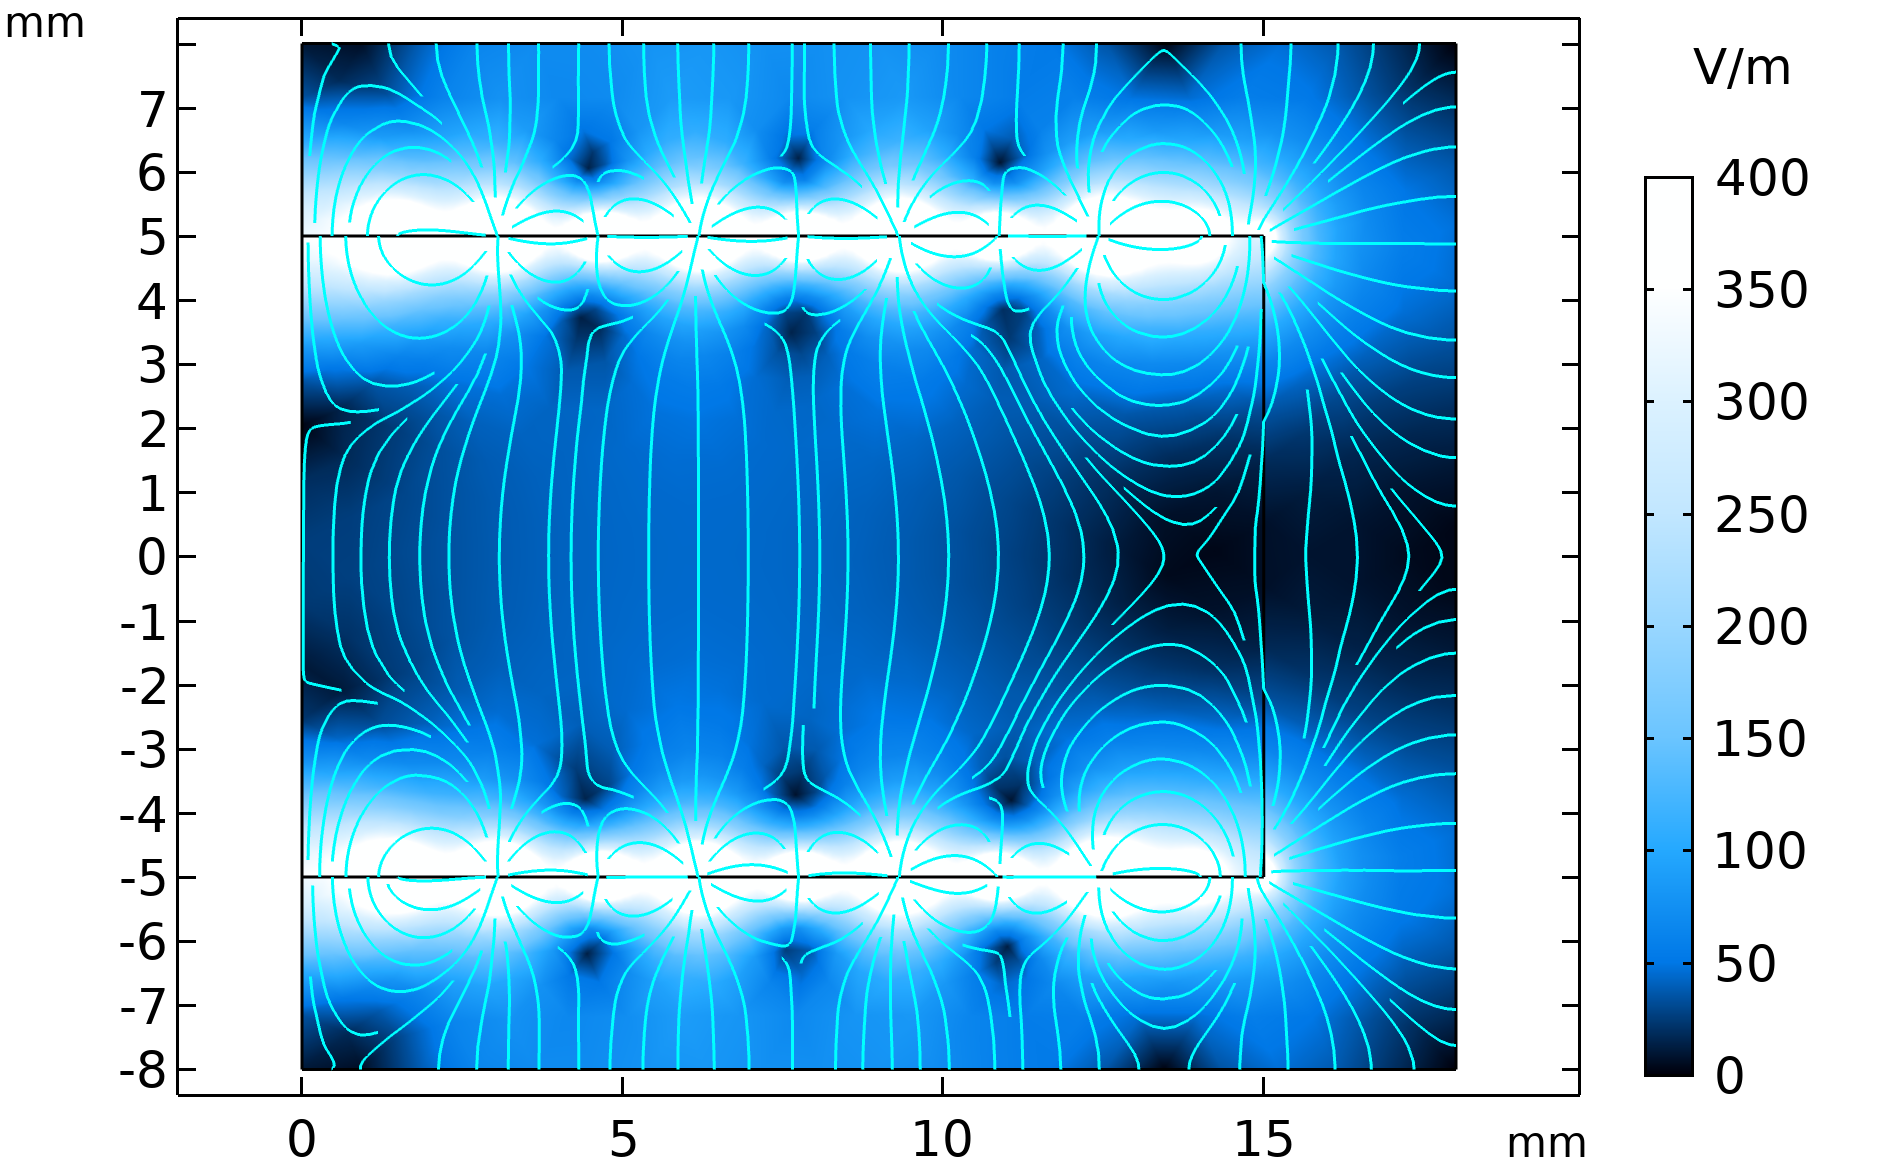
\includegraphics[align=c, scale=0.5]{Figures/ElectrodesExperimental/efield_redn1.png}
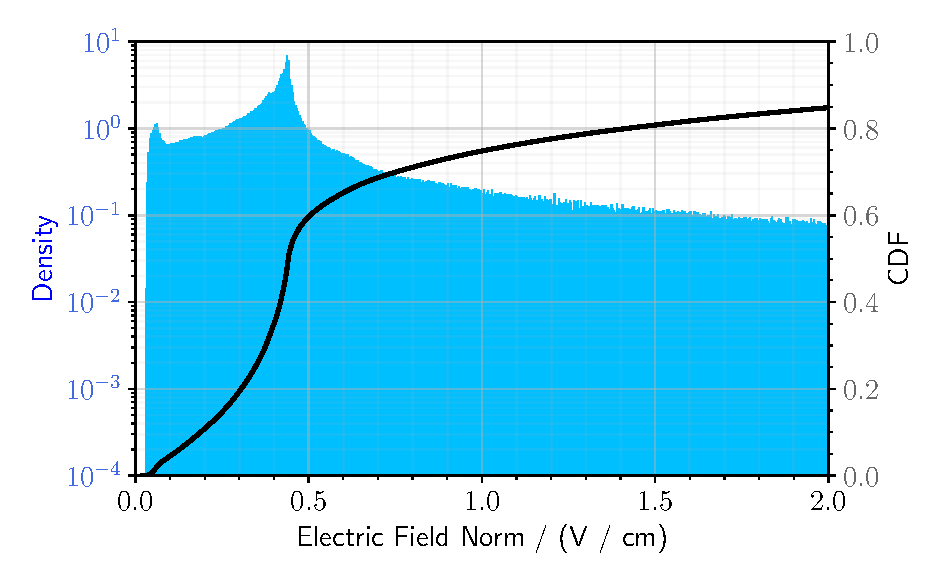
\includegraphics[align=c, scale=0.5]{Figures/ElectrodesExperimental/enorm_hist_redn1.pdf}
\caption{(On the left) Color map of the magnitude of the electric field with white representation of the electric field lines from the simulation of REDN1. The default polarization is used. The colored volumes in the scheme \ref{fig:redn1-scheme} are drawn from the electric field lines with common start and end points.
(On the right) Histogram and Cumulative Distribution Function of the distribution of the magnitude of the electric field over the crystal volume from the simulation of REDN1.}
\label{fig:redn1-efield}
\end{figure}

% Scan over R_veto
In the later paragraph \ref{par:redn1-comparison}, the REDN1 simulation is compared to the experimental data taken during the operation of REDN1. Specifically, two distinct scans were conducted over the the voltage bias $V_{bias}$ and the polarization ratio $R_{veto}$. As discussed in the previous chapter \ref{ChapterElectrodesScan}, leaves all the quantities evaluated from the simulation of REDN1 unaffected except for a scaling of the magnitude of the electric field.
However, scanning over $R_{veto}$ induces changes on the fiducial volume and the electric field. Therefore, this scan was conducted with the REDN1 simulation as to compare with experimental data later. The scan is performed over a linear scale from \SIrange{0}{1}{} with the defalut configuration being $R_{veto} = 0.4$. The results are presented as graphs in the figure \ref{fig:redn1-scan}. The top graph corresponds to the fiducial volume percentage $\%_{fid}$ while the bottom graph displays some percentiles $f_x$ of the electric field magnitude distribution. 
The grey-shaded range from $0$ to $0.375$ indicates that fiducial field lines are in contact with the lateral surface of the crystal. Such a configuration is expected to have adversarial effects on the surface tagging ability of the detector, as discussed in paragraph \ref{par:fid38-veto-ratio}.
The red-shade range for $R_{veto} > 0.925$ indicates that the fiducial values were overestimated due to the unexpected integration of some veto volume. As such, the percentages should not be considered.
The global trend of the fiducial percentage is a significant decrease with the rising $R_{veto}$. Indeed, as this parameter increases, the veto volumes grows deeper into the bulk of the crystal. This observation is on par with the decrease in the electric field norm in the crystal. This is due to the potential of the veto electrodes increases in absolute value with $R_{veto}$ up to $0.6$. From this point onward, the median magnitude greatly recovers while other percentiles $f_{x \leq 0.25}$ see their value lower and stabilize. Indeed, with the ever decreasing fiducial volume, the veto and equatorial volume grows significantly in size and field strength. On the contrary, the bulk volume shrinks and has a lowered field strength.

\begin{figure}
\centering
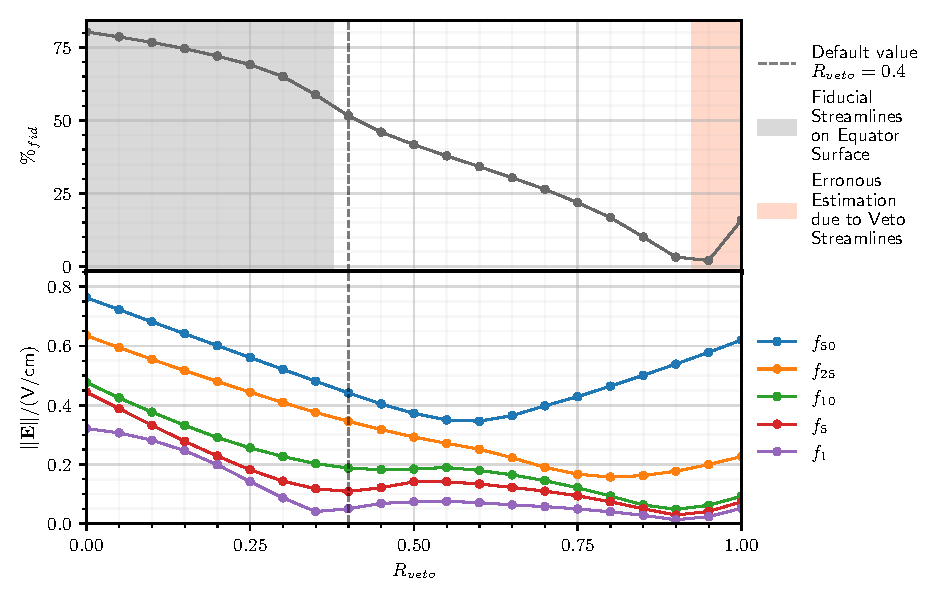
\includegraphics[scale=1]{Figures/ElectrodesExperimental/redn1_scan_veto_ratio.pdf}
\caption{Scan over the polarization ratio parameter $R_{veto}$ from the simulation of REDN1. The plotted quantities are the fiducial volume percentage $\%_{fid}$ and some percentiles $f_x$ of the electric field norm. The red area indicates an overestimation of the fiducial volume through the erroneous integration of veto volume in the used algorithm. Fiducial percentage is this area should not be considered.}
\label{fig:redn1-scan}
\end{figure}


\section{Detector Operation and Analysis Pipeline}


\subsection{Experimental Setup}

The detectors RED80 and REDN1 were studied in two separate cryostat runs: the Run 57 and 61 respectively. In each of the runs, detectors were placed in the suspended tower described in paragraph \ref{par:suspended-tower}. The germanium crystals of the detectors were activated with the AmBe neutron source as described in paragraph\ref{par:calibration-source}. As such, RED80 and REDN1 are operated with an intrinsic calibration peak of \SI{10.37}{\kilo\eV} electronic recoils with uniform distribution over the detector volume. The data collection consists in multiple streams with different ionization channel configurations. Each streams is at least 2 hours long as to explore enough configuration points while gathering enough statistics for the analysis. Some occasional streams are longer as taken during nights and weekends. Some ionization configuration were repeated and can be used to estimate the reproducibility of the measurements. The streams along with their corresponding polarization configuration are listed in the tables \ref{tab:red80-stream-list} for RED80 and \ref{tab:redn1-stream-list} for REDN1.
The detector RED80 was operated in the Run 57 along with the detector RED70 based on the FID38 design. Although it was based on the FID38 design, RED70 showed very high leakage currents between the electrodes, even at very low voltage bias $V_{bias} \approx \SI{0.1}{\volt}$. Such currents leads to a huge increase in temperature and a quick saturation of the ionization electronics. As such, RED70 is virtually unusable with polarized electrodes, and is not studied in this work. The detector RED80 was operated with two different heat channel configuration. Before and up to the stream tg17l000, RED80 was regulated at the temperature $T_{cryo}=\SI{18}{\milli\kelvin}$ with a bias current $I_{bias} = \SI{2}{\nano\ampere}$ through its NTD of resistance $R_{NTD}=\SI{1.6}{\mega\ohm}$. From and after the stream tg17l001, the regulation temperature was decreased to $T_{cryo}=\SI{16}{\milli\kelvin}$ with a bias current $I_{bias} = \SI{1}{\nano\ampere}$ with the NTD resistance measured at$R_{NTD}=\SI{3.8}{\mega\ohm}$.
As addressed in paragraph \ref{par:charge-drifting}, the ionization channel performances are independent from the configuration of the heat channel. So, in the case of RED80, the comparison of stream with different current bias $I_{bias}$ of the NTD is valid.
The detector REDN1 was operated along with the detector RED90 in the Run 61. RED90 is used for NTD characterization like the RED detectors used in chapter \ref{ChapterEthemExperimental}. It consists in a germanium crystal with a bare surface and a single NTD thermal sensor and does not possess an ionization channel.
The temperature of the detector REDN1 is regulated at the temperature $T_{cryo}=\SI{14}{\milli\kelvin}$ for the whole run with a single configuration of its heat channel: the bias current was set to $I_{bias}=\SI{0.54}{\nano\ampere}$ through the NTD of resistance $R_{NTD} = \SI{6.6}{\mega\ohm}$.

\begin{table}[]
\centering
\begin{tabular}{c|rrr}
\multicolumn{1}{c|}{\multirow{2}{*}{Stream}} & \multicolumn{1}{c}{\multirow{2}{*}{$V_{bias}$/ V}} & \multicolumn{2}{|c}{Polarization / V}              \\ \cline{3-4} 
\multicolumn{1}{c|}{}                        & \multicolumn{1}{c|}{}                               & \multicolumn{1}{c|}{$A,B$} & \multicolumn{1}{c}{$C,D$} \\ \hline \hline
tk18l001 & -4   & -2    & +2    \\ \hline
tk19l001 & -2   & -1    & +1    \\ \hline
tk19l000 & -1   & -0.5  & +0.5  \\ \hline
tk18l000 & -0.5 & -0.2  & +0.2  \\ \hline
tk15l005 & -0.2 & -0.1  & +0.1  \\ \hline
tk15l005 & -0.1 & -0.05 & +0.05 \\ \hline
tk20l000                                     & \multirow{2}{*}{0.1}                                & \multirow{2}{*}{0.05}    & \multirow{2}{*}{-0.05}  \\
tk25l000 &      &       &       \\ \hline
tk25l001 & 0.2  & +0.1  & -0.1  \\ \hline
tk27l001 & 0.5  & +0.2  & -0.2  \\ \hline
tk26l001 & 1    & +0.5  & -0.5  \\ \hline
tk26l000 & 2    & +1    & -1    \\ \hline
tk20l003 & 4    & +2    & -2   
\end{tabular}%
\caption{List of the streams with their polarization for the experimental study of RED80 in the Run 57.}
\label{tab:red80-stream-list}
\end{table}

\begin{table}[]
\centering
\begin{tabular}{c|rrrrrr}
\multicolumn{1}{c|}{\multirow{2}{*}{Stream}} &
  \multicolumn{1}{c|}{\multirow{2}{*}{$V_{bias}$/ V}} &
  \multicolumn{1}{c|}{\multirow{2}{*}{$R_{veto}$}} &
  \multicolumn{4}{c}{Polarization / V} \\ \cline{4-7} 
\multicolumn{1}{c|}{} &
  \multicolumn{1}{c|}{} &
  \multicolumn{1}{c|}{} &
  \multicolumn{1}{c|}{$A$} &
  \multicolumn{1}{c|}{$B$} &
  \multicolumn{1}{c|}{$C$} &
  \multicolumn{1}{c}{$D$} \\ \hline \hline
tk18l001					  & -2                 & 0.4                  & +0.4                  & -1                  & -0.4                  & +1                  \\ \hline
tk19l001                      & 0.25               & 0.4                  & -0.05                 & +0.125              & +0.05                 & -0.125              \\ \hline
tk19l000                      & 0.5                & 0.4                  & -0.1                  & +0.25               & +0.1                  & -0.25               \\ \hline
tk18l000                      & 1                  & 0.4                  & -0.2                  & +0.5                & +0.2                  & -0.5                \\ \hline
tk15l005                      & \multirow{2}{*}{2} & \multirow{2}{*}{0.4} & \multirow{2}{*}{-0.4} & \multirow{2}{*}{+1} & \multirow{2}{*}{+0.4} & \multirow{2}{*}{-1} \\
tk15l005                      &                    &                      &                       &                     &                       &                     \\ \hline
tk20l000                      & \multirow{2}{*}{4} & \multirow{2}{*}{0.4} & \multirow{2}{*}{-0.8} & \multirow{2}{*}{+2} & \multirow{2}{*}{+0.8} & \multirow{2}{*}{-2} \\
tk25l000                      &                    &                      &                       &                     &                       &                     \\ \hline
tk25l001  & 8                  & 0.4                  & -1.6                  & +4                  & +1.6                  & -4                  \\ \hline \hline
tk27l001                      & 4                  & 0.2                  & -0.4                  & +2                  & +0.4                  & -2                  \\ \hline
tk26l001  & 4                  & 0.3                  & -0.6                  & +2                  & +0.6                  & -2                  \\ \hline
tk26l000  & 4                  & 0.5                  & -1                    & +2                  & +1                    & -2                  \\ \hline
tk20l003  & 2                  & 0.6                  & -0.6                  & +1                  & +0.6                  & -1                  \\ \hline
tk27l002  & 4                  & 0.7                  & -1.4                  & +2                  & +1.4                  & -2                 
\end{tabular}%
\caption{List of the streams with their polarization for the experimental study of REDN1 in the Run 61.}
\label{tab:redn1-stream-list}
\end{table}


\subsection{Quality Cuts}
%\label{par:quality-cuts}

{\color{red} Might move the explanation of the processing and quality cuts in this chapter. To be discussed. For now, it is essential to write about the specifics of RED80 and REDN1.

TO DO: merge with Quality Cuts from Chapter Neutron
}

The data collection and processing is describe in the later chapter \ref{ChapterNeutron} dedicated to the "Neutron Analysis with RED80". This paragraph presents the specific quality cuts used for the analysis of the data from RED80 and REDN1.

% Livestream cut
The live stream cut described in paragraph \ref{par:livestream-cut} is not applied in this chapter. Indeed, the comparison of the simulation of RED80 and REDN1 to the experiment is not based on the rate of events. As to ease the workload of analysis, this cut is not applied.

% Maintenance and Reset Cut
The maintenance and reset cut presented in paragraph \ref{par:maintenance-reset-cut} is used in the analysis of RED80 and REDN1 with the same tolerance parameters.

% Offset Cut
The offset cut is applied as described in the paragraph \ref{par:offset-cut}. The same threshold $A_{offset}=\SI{14000}{ADU}$ is used.

% Chi2 cuts
The $\chi^2$ cuts are applied in the same fashion as described in the paragraph \ref{par:chi2-cuts}. All the events with any estimated $\chi^2$, on the heat channel or one of the ionization channels, above a defined threshold function is discarded from the analysis.
The threshold is a function of the signal amplitude $A_X$ of a channel $X$ in ADU. Its expression is
\begin{equation}
\chi_{threshold}^2 (A_X) = \chi_0^2 \cdot \left( 1 + \left( \frac{A_X}{A_0} \right)^b \right)
\end{equation}
depending on the three parameters: the baseline threshold $\chi_0^2$, the takeoff amplitude $A_0$ and the quadratic factor $b$.

\begin{table}[]
\centering
\begin{tabular}{c|l|c|c|c}
Detector               & Channel & $\chi_0^2$                & $A_0$                      & $b$ \\ \hline \hline
\multirow{2}{*}{RED80} & Heat    & \multirow{2}{*}{400}      & \num{3e3} & 2   \\ \cline{2-2} \cline{4-5} 
 &
  \begin{tabular}[c]{@{}l@{}}Ionization\\ $A,B,C,D$\end{tabular} &
   &
  \multicolumn{1}{r|}{\num{2e3}} &
  \multicolumn{1}{r}{2.2} \\ \hline \hline
REDN1                  & Heat    & \multicolumn{1}{r|}{2000} & \num{3e3} & 2   \\
tk19l000 &
  \begin{tabular}[c]{@{}l@{}}Ionization\\ $A,B,C,D$\end{tabular} &
  \multicolumn{1}{r|}{700} &
  \multicolumn{1}{r|}{\num{2e3}} &
  \multicolumn{1}{r}{2.2}
\end{tabular}%
\caption{Parameters for the quality cuts used in the RED80 and REDN1 data analysis.}
\label{tab:red80-redn1-quality-cuts}
\end{table}


\subsection{Cross-talk correction and Cabling capacitance estimation}

The paragraph \ref{par:sensitivity-calculation} discuss the expression of the signal induced on the ionization channel by a recoil. It is demonstrated that a recoil, creating a number $N_p$ of electron-hole pairs, generates a charge perturbation on the electrodes $A$ through $D$. This perturbation is expressed as the charge perturbation vector $\vec{Q}$. In the case of the REDN1 and RED80, there are different charge perturbation vector depending on the recoil location in the crystal. Their expression are displayed in equation \ref{eq:red80-induced-charges} for RED80 and \ref{eq:fid38-induced-charges} for REDN1, considering an ideal drift of the charges and a complete collection on the electrodes.
The voltage signal $\vec{V}$ generated on the electrode is calculated from the charge vectors and the Maxwell capacitance matrix $C$ of the detector according to the equation \ref{eq:capacitance-definition-matrix}. It is calculated in the equations \ref{eq:planar38-sensitivity} for the PL38 design and the equations \ref{eq:fid38-sensitivity} for the FID38 design. Contrary to the charge vector $\vec{Q}$ which has 2 null component, a voltage signal is generated on all the electrodes of the detector. This phenomenon is called cross-talk.
The cross-talk correction is an analysis step consisting in calculating an effective charge vector $\vec{Q}_{eff}$ corresponding to a measured voltage signal vector $\vec{V}_{meas.}$. With cross-talk corrected measurement, it is possible to proceed with the calibration of the detector and the rest of the analysis.
The calculation is done with the cross-talk correction matrix $\bm{C}_{X-talk}$ such that:
\begin{equation}
\vec{Q}_{eff} = \bm{C}_{X-talk} \cdot \vec{V}_{meas.}
\end{equation}
This equation is the experimental equivalent of the equation \ref{eq:capacitance-definition-matrix} dedicated to theoretical perturbation vector $\vec{Q}$ and $\vec{V}$ on a detector of known Maxwell capacitance matrix $\bm{C}$. As a result, the cross-talk correction matrix is equal to the Maxwell capacitance matrix of the detector and the cabling such that:
\begin{equation}
\bm{C}_{X-talk} = \bm{C}_{total} = \bm{C}_{detector} + \bm{C}_{cabling} 
\end{equation}
The Maxwell capacitance matrix of the detector $\bm{C}_{detector}$ is considered known as it is yielded from the detector simulation in the equations \ref{eq:red80-maxwell} and \ref{eq:redn1-maxwell} for RED80 and REDN1 respectively.
The paragraph \ref{par:sensitivity-calculation} explains that the cabling possesses a diagonal Maxwell capacitance matrix. Under the assumption that the properties of the cabling, like its length or its shielding, is the same for all the electrodes, all its diagonal components are equals. Their value is a single cabling capacitance $C_{cabling}$ which is unknown.
Therefore, all the non-diagonal terms of the cross-talk correction $C_{X-talk}$ matrix are known and its diagonal terms are to be defined through the estimation of the cabling capacitance $C_{cabling}$.

This estimation is based on the expected charge perturbation vector $\vec{Q}_{bulk}$ from the fully collected bulk event created in by the calibration electronic recoil at \SI{10.37}{\kilo\eV}. This estimation process is therefore iterative as cross-talk correction and energy calibration are interdependent. 
For this analysis, the cross-talk correction is first approximated with a graphical method. The calculated effective charge signal $\vec{Q}_{eff}$ are then used in the calibration step, described in the following paragraph \ref{par:calibration-step}, and in the selection of the calibration events described in the paragraph \ref{par:calibration-events-selection}. The precise cross-talk correction is effectuated with the \SI{10.37}{\kilo\eV} calibration events only and the analysis pipeline is re-run with this additional precision.

% Graphical method
The cross-talk correction matrix $\bm{C}_{X-talk}$ and more specifically the cabling capacitance $C_{cabling}$, are approximated with a graphical method. The principle is to have the effective charge perturbation vector $\vec{Q}_{eff}$ correspond to the theoretical charge perturbation vectors $Q$ for the different collection volume: bulk, guard, veto as expressed in equations \ref{eq:red80-induced-charges} and \ref{eq:redn1-induced-charges}. As the detector is not calibrated yet, the component of the theoretical charge vector are known up to a calibration factor $a_X$ depending on the electrode $X$. Considering the bulk events of RED80 as reference, the equation that is solved graphically with $C_{cabling}$ as unknown is the following:
\begin{equation}
\label{eq:crosstalk-correction}
\textsf{diag}(a_A, a_B, a_C, a_D)
\cdot
\vec{Q}_{bulk}
=
\begin{bmatrix}
0 \\ -a_B \\ 0 \\ a_D
\end{bmatrix} 
=
\left( \bm{C}_{detector} + C_{cabling} \cdot \mathbb{1} \right) \cdot \vec{V}_{meas., bulk}
\end{equation}

As the calibration coefficient $a_X$ are unknown, it is handy to consider a normalized cross-talk corrected signal vector $\vec{Y}$ expressed as:
\begin{equation}
\vec{Y}^{bulk} \left( C_{cabling} \right)
=
\frac{1}{C_{detector, 11} + C_{cabling}}
\left( \bm{C}_{cabling} + C_{cabling} \cdot \mathbb{1} \right) \cdot \vec{V}_{meas., bulk}
= \bm{C}_{X-talk}^N \cdot \vec{V}_{meas., bulk}
\end{equation}
with $\bm{C}_{X-talk}^N$ the normalized cross-talk correction matrix.

With a correctly estimated $C_{cabling}$ satisfying the equation \ref{eq:crosstalk-correction}, the cross-talk corrected signal vector $\vec{Y}^{bulk}$ of the bulk event has two null components $Y_A^{bulk} = Y_C^{bulk} = 0$ and two non-null components $Y_B^{bulk}$ and $Y_D^{bulk}$.
In order to visualize the four components of the cross-talk corrected vector $\vec{Y}$ visualization, corner plots are used . The figure \ref{fig:red80-crosstalk-correction} present such a corner plot for the detector RED80 for the stream tg09l000 in the Run 57. Only events passing the quality cuts are plotted. The dashed guide lines indicates the null signal at \SI{0}{ADU} and the full collection of the \SI{10.37}{\kilo\eV} calibration electronic recoils  at $\approx \pm \SI{55}{ADU}$ (drawn a fortiori after the calibration step).
Each color corresponds to a different cabling capacitance value $C_{cabling}$ with the vector $\vec{Y}(\SI{125}{\nano\farad})$ colored in orange, $\vec{Y}(\SI{0}{\nano\farad})$ colored in green and $\vec{Y}(+\infty)$ colored in blue. We note that as $C_{cabling} \rightarrow +\infty, \ \bm{C}_{X-talk}^N \rightarrow \mathbb{1}$. The non-diagonal terms of the normalized cross-talk correction matrix $\bm{C}_{X-talk}^N$ are inversely proportional to the cabling capacitance $C_{cabling}$. As a result, we observe a diminishing return in the change of shape of the vector $\vec{Y}$ with increasing $C_{cabling}$.

\begin{figure}
\centering
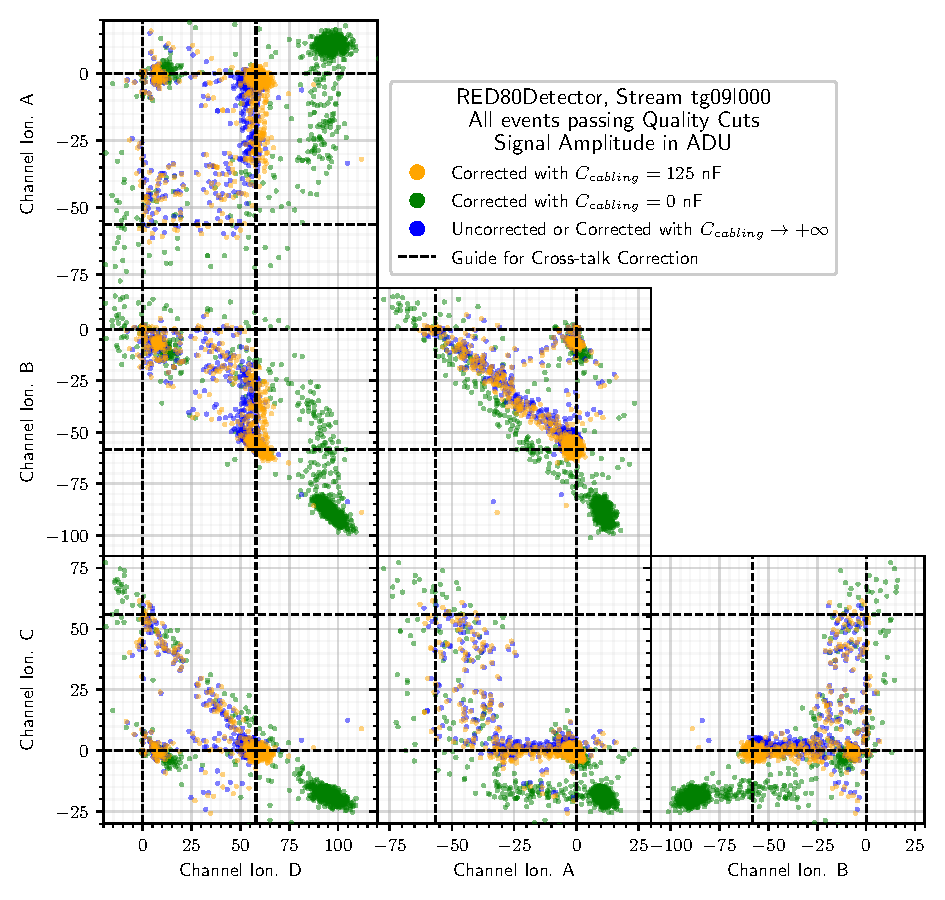
\includegraphics[scale=1]{Figures/ElectrodesExperimental/red80_crosstalk_correction.pdf}
\caption{Corner plot of the cross-talk corrected amplitude vector $\vec{Y}$ in ADU. The plotted events belong corresponds to the stream tg09l000 of the run 57 operating the detector RED80. Only events passing the quality cuts are displayed. Each color corresponds do a different cabling capacitance $C_{cabling}$ used to calculate the cross-talk correction matrix $\bm{C}_{X-talk}$. The guide lines indicate no collection at \SI{0}{ADU} and full collection at $\approx \pm \SI{55}{ADU}$ of the \SI{10.37}{\kilo\eV} calibration electronic recoils.}
\label{fig:red80-crosstalk-correction}
\end{figure}

The correct cabling capacitance $C_{cabling}$ satisfying the equation \ref{eq:crosstalk-correction} is chosen when the distribution of the components of $\vec{Y}$ in the corner plots mostly corresponds to the guide lines.
In the case of $RED80$ and $REDN1$, the cabling capacitance was first estimated to $C_{cabling} = \SI{120}{\nano\farad}$. 
We  can check that the normalized cross-talk correction matrix $\bm{C}_{X-talk}^N$ corresponds to the identity matrix at the first order. The correction terms are in the range of few percents, going up to $5.2\%$ in the case of the case of the electrode $B$ inducing signal on the electrode $A$.

% Precise estimation
The precise estimation of the cabling capacitance $C_{cabling}$ and the cross-talk correction matrix $\bm{C}_{X-talk}$ happens after the calibration step and the selection of the full collected bulk events created by the \SI{10.37}{\kilo\eV} calibration electronic recoils.
A fiducial recoil leads to an electric charge perturbation expresses by the vector $\vec{Q}$ such that:
\begin{equation}
\vec{Q}_{fid}^{REDN1} =
\begin{bmatrix}
0 \\ -1 \\ 0 \\ 1
\end{bmatrix}
\cdot Q(\SI{10.37}{\kilo\eV})
\end{equation}
with the electric charge multiplicative factor being:
\begin{equation}
Q(\SI{10.37}{\kilo\eV})
=
N_p(\SI{10.37}{\kilo\eV}) \cdot e
=
\frac{E_R}{\epsilon} e
=
\frac{\SI{10.37e3}{\eV}}{\SI{3}{\eV}} e
\end{equation}

According to equation \ref{eq:matrix-capacitance-charge}, the voltage signal induced on the electrodes is expressed by the vector $\vec{V}_{fid}^{REDN1}$ obtained with the Maxwell capacitance matrix  of the detector and cabling $\bm{C}_{total} = \bm{C}_{detector} + \bm{C}_{cabling}$ such that:
\begin{equation}
\label{eq:redn1-bulk-voltage-vector}
\vec{V}_{fid}^{REDN1}
=
\begin{bmatrix}
V_A \\ V_B \\ V_C \\ V_D
\end{bmatrix}
=
\bm{C}_{total}
\cdot
\vec{Q}_{fid}^{REDN1}
\end{equation}

In the paragraph \ref{par:sensitivity-calculation}, the Maxwell capacitance matrix associated with the cabling $\bm{C}_{cabling}$ is considered to be diagonal with $\forall i \neq j, \bm{C}_{cabling, ij} = 0$ . The previous equation \ref{eq:redn1-bulk-voltage-vector} can be translated for the terms $\bm{V}_{i}$ and $\bm{Q}_i$ of the vectors $\vec{V}_{fid}^{REDN1}=\vec{V}$ and $\vec{Q}_{fid}^{REDN1}=\vec{Q}$ respectively:
\begin{align}
\bm{V}_{i}
&=
\sum_{j=1}^4 \bm{C}_{total, ij} \bm{Q}_j
\\
&=
\sum_{j=1}^4 \bm{C}_{detector, ij} \bm{Q}_j + \sum_{j=1}^4 \bm{C}_{cabling, ij} \bm{Q}_j
\\
&=
\left(
 \bm{C}_{detector, i4} - \bm{C}_{detector, i2}
\right)
Q(\SI{10.37}{\kilo\eV}) + \bm{C}_{cabling, ii} \bm{Q}_i
\end{align}

We assume that the Maxwell capacitance matrix relative to the detector $\bm{C}_{detector}$ is known as it calculated from the electrostatics simulation of REDN1. The diagonal terms $\bm{C}_{cabling, ii}$ of the cabling capacitance matrix can therefore be evaluated from the voltage signal induced by the \SI{10.37}{\kilo\eV} fiducial events $\bm{V}_{i}$ :
\begin{equation}
\label{eq:cabling-capacitance-expression}
\bm{C}_{cabling, ii}
=
\frac{1}{\bm{Q}_i} \left[ \bm{V}_{i} - \left( \bm{C}_{detector, i4} - \bm{C}_{detector, i2} \right) Q(\SI{10.37}{\kilo\eV}) \right]
\end{equation}

One should note that as $\bm{Q}_1 = \bm{Q}_3 = 0$, the equation \ref{eq:cabling-capacitance-expression} is only valid for $i \in \{ 2,4 \}$. This means that the fiducial events collected by the electrode $B$ and $D$ can only be used to determine the cabling capacitance associated with these very electrodes $\bm{C}_{cabling, 22}$ and $\bm{C}_{cabling, 44}$ respectively.

\begin{figure}
\centering
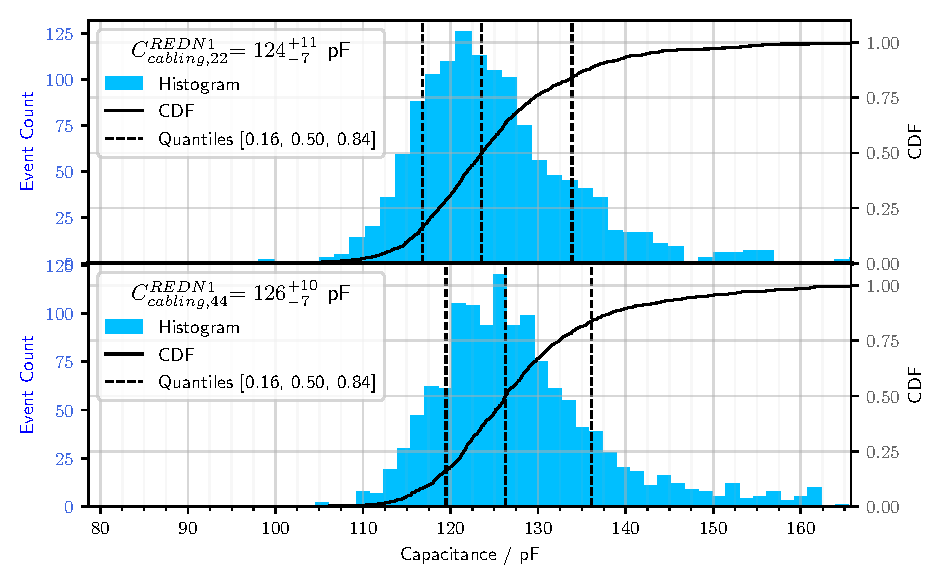
\includegraphics[scale=1]{Figures/ElectrodesExperimental/redn1_cabling_capacitance_fitting.pdf}
\caption{Fitting the cabling capacitance for REDN1.}
\label{fig:red80-cabling-capacitance}
\end{figure}

\begin{figure}
\centering
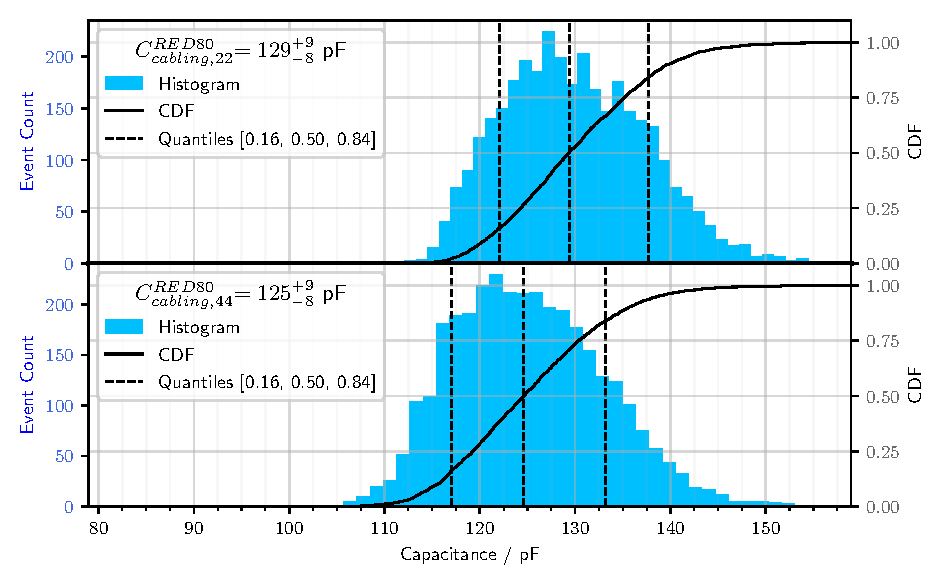
\includegraphics[scale=1]{Figures/ElectrodesExperimental/red80_cabling_capacitance_fitting.pdf}
\caption{Fitting the cabling capacitance for RED80.}
\label{fig:red80-cabling-capacitance}
\end{figure}

{\color{red} Description of the histograms, conclusion on the 125 nF, the more complex model with one cabling capacitance for each electrode of the ionization channel.
Interpret the difference between detectors as being small variation in length of the cabling between the conductive tracks on the copper chassis in the suspended tower and the electronics on the fixed mixing chamber of the cryostat.

TO DO: merge with X-talk from Chapter Neutron
}


\subsection{Calibration}

{\color{red} Calibration is done as described in the paragraph \ref{par:calibration}.

TO DO: merge with Calibration from Chapter Neutron}

%The paragraph \ref{par:data-processing} describes how a signal amplitude is associated to each event in the stream. The unit of this signal amplitude is ADU. In the case of the heat channel, the signal amplitude is proportional to the heat energy $E_{heat}$ of an event. For the ionization channel, it is the electric charge $Q_X$ that is induced on an electrode $X$ that is proportional to the signal amplitude measured by the electrode.
%The voltage signal $\vec{V}$ is measured as the signal amplitude in ADU with a factor conversion of \SI{67.4}{\nano\volt\per\kilo\eV}. 


\subsection{Fiducial Cut}


{\color{red} The fiducial cuts are done as described in the paragraph \ref{par:fiducial-cuts}. With a broader range for the selection for the population.

- Incomplete vs Full collection: 3 sigma of the resolution at 10.37 keV.
- Bulk cut: 5 sigma of the baseline resolution.

TO DO: merge with Fiducial-cut from Chapter Neutron
}


\section{Experimental Estimation of the Fiducial Volume and Comparison to the Detector Simulation}

\subsection{Control values definition}

-For each detector RED80 and REDN1

-For each stream

-Selection of events passing the quality cuts produced by \SI{10.37}{\kilo\eV} calibration electronic recoils.

- $n_{tot}$: total number of such events in a stream. This number is assumed to part of the Poisson distribution, thus the statistical error is $\sigma^2 (n_{tot}) = n_{top}$

- $n_{incomplete}$: number of incomplete events. This number is subject to a binomial distribution. the statistical error is 
\begin{align}
\sigma^2 (n_{incomplete} )
&=
n_{tot} \cdot p \cdot (1-p)
\\
&=
n_{tot} \cdot \frac{n_{incomplete}}{n_{total}} \cdot \left( 1 - \frac{n_{incomplete}}{n_{total}}  \right)
\\
&= 
n_{incomplete} \cdot \left( 1 - \frac{n_{incomplete}}{n_{total}}  \right)
\end{align}

- $n_{complete} = 1 - n_{incomplete} $: number of complete collection events. Same error as $n_{incomplete}$.

- $n_{bulk}$: number of bulk events chosen among complete collection events. Subject to binomial distribution with an error :
\begin{equation}
\sigma^2 (n_{bulk} )
= 
n_{bulk} \cdot \left( 1 - \frac{n_{bulk}}{n_{incomplete}}  \right)
\end{equation}

- The incomplete percentage is expressed $\frac{n_{incomplete}}{n_{total}}$ and the statistical error on this ratio is:
$$ error propagation $$
%\begin{align}
%\sigma^2 \left( \frac{n_{incomplete}}{n_{total}} \right)
%&=
%\frac{1}{n_{tot}^2} \cdot \sigma^2 (n_{incomplete})
%+ 
%\left( \frac{n_{incomplete} }{n_{tot}^2} \right)^2 \cdot \sigma^2 (n_{tot})
%\\
%&=
%\left( 
%	\frac{n_{incomplete}}{n_{total}}
%\right)^2 
%\cdot 
%\left[ 
%	\left(
%		1 - \frac{ n_{incomplete} }{ n_{total} }
%	\right)^2 
%	+ \frac{ 1 }{ n_{tot} }
%\right]
%\end{align}


- Efficiency percentage is expressed $\frac{n_{bulk}}{n_{total}}$ with the same statistical error.

- Fiducial percentage is expressed $\frac{n_{bulk}}{n_{complete}}$ with the statistical error being:
$$ error propagation $$
%\begin{align}
%\sigma^2 \left( \frac{n_{bulk}}{n_{complete} \right)
%&=
%\left( \frac{\sigma (n_{bulk})}{n_{complete}} \right)^2 + \left( \frac{n_{bulk} \cdot \sigma (n_{complete})}{n_{complete}^2} \right)^2
%\\
%&=
%\left( \frac{n_{bulk}}{n_{incomplete} \right)^2 \cdot \left[ \left( 1 - \frac{n_{bulk}}{n_{complete}}  \right)^2 + \left( 1 - \frac{n_{complete}}{n_{total}}  \right)^2 \right]
%\end{align}
%

\subsubsection{RED80}

\begin{figure}
\centering
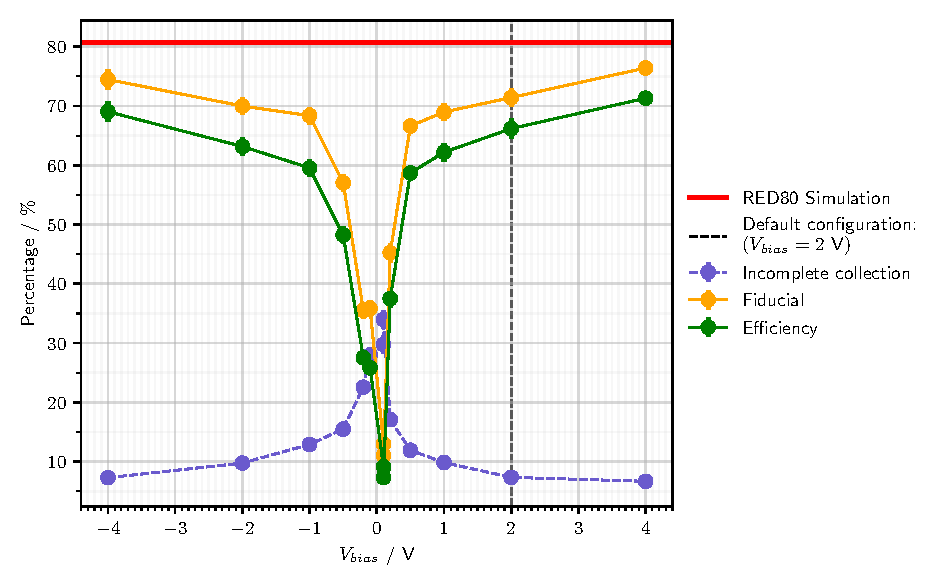
\includegraphics[scale=1]{Figures/ElectrodesExperimental/red80_experimental_fiducial_volume.pdf}
\caption{Experimental percentages of incomplete collection (in blue), of fiducial events (in orange) and of the efficiency (in green) as functions of the voltage bias $V_{bias}$ for the detector RED80. The theoretical fiducial volume percentage $\%_{fid}=\SI{80.75}{\percent}$ estimated with the RED80 simulation is indicated by the horizontal red line. \\
{\color{red} TODO: correct the error bars}
}
\label{fig:red80-experimental-fiducial-volume}
\end{figure}

- All the control values are presented for RED80 as functions of the $V_{bias}$ in the figure \ref{fig:red80-experimental-fiducial-volume}. (full description...)

- Apparent seagull profile shape of the curves

- Symmetry between negative and positive $V_{bias}$ seems respected within the errors bars.

- The experimental fiducial volume at least lower by $10\%$ from the theoretical volume estimated from the RED80 simulation. Due to frontier events with a non-negligeable (greater than 5 sigma) induced on the guard electrodes $A$ or/and $C$. Visible on the corner plot, especially for the electron-collecting electrodes (for tg09l009, $A$ and $B$) as they are effected with transversal movement in the crystal.

- The experimental fiducial volume tends to the theoretical fiducial volume for the highest absolute of $V_{bias}$. A higher electric field magnitude negates the transversal movement of the charges which follow more closely the field lines.

- The incomplete charge collection has a low caps for $| V_{bias} | \geq \SI{2}{\volt}$ at a percentage of about \SI{8}{\percent}. For lower absolute value of the voltage bias, the incomplete percentage significantly rises. This divergence of the incomplete percentage is consistent with the absence of collection at $V_{bias}=\SI{0}{\volt}$ as the electrodes are not polarized and the electron-hole pairs recombine in the crystal.

- Good efficiency between 1 and 4 volts with an efficiency percentage between 62 and 72 percents. The default polarization at $V_{bias} = \SI{2}{\volt}$.


\subsubsection{REDN1}

\begin{figure}
\centering
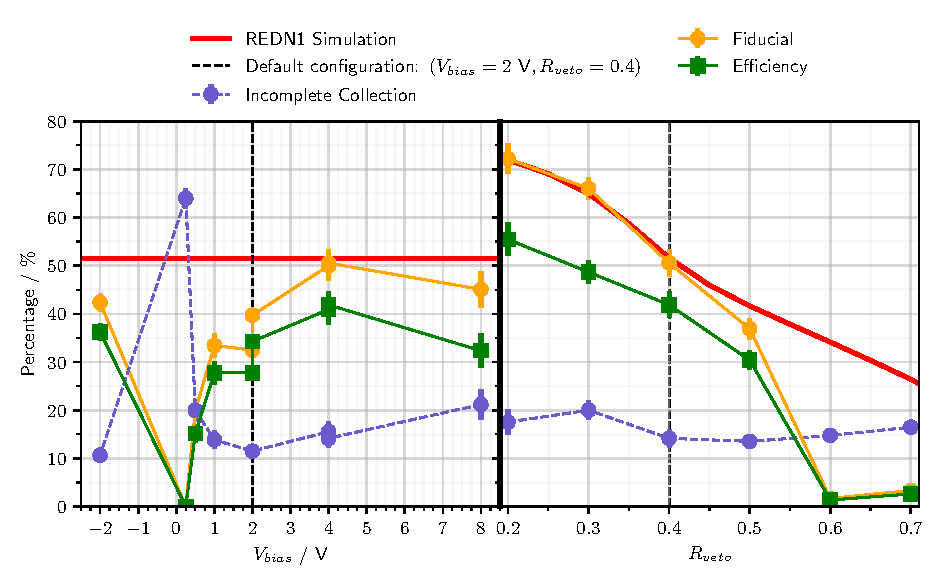
\includegraphics[scale=1]{Figures/ElectrodesExperimental/redn1_experimental_fiducial_volume.pdf}
\caption{Experimental percentages of incomplete collection (in blue), of fiducial events (in orange) and of the efficiency (in green) as functions of the voltage bias $V_{bias}$ (on the left) or of the polarization ratio $R_{veto}$ (on the right) for the detector REDN1. The theoretical fiducial volume percentage estimated with the REDN1 simulation is indicated by the red lines. \\
{\color{red} TODO: correct the error bars}}
\label{fig:redn1-experimental-fiducial-volume}
\end{figure}

- All the control values are presented for REDN1 as functions of the $V_{bias}$ in the figure \ref{fig:redn1-experimental-fiducial-volume} on the left. (full description...)

- The seagull profile is still present, with high fiducial volume at higher $V_{bias}$

- Again, divergence of the incomplete charge collection at low voltage bias.

- Good correspondence of the percentages between $2$ and $-2$ of $V_{bias}$.

- For $V_{bias}=\SI{4}{\volt}$, the  experimental fiducial volume is greater than predicted by the simulation. Although, still in the error bars.

- Need to investigate the high bias value $V_{bias} = \SI{8}{\volt}$ with a drop in fiducial volume and efficiency. Not explained for now.

- The redundant configuration $V_{bias} = \SI{2}{\volt}$ displays a difference of almost \SI{10}{\percent} between the fiducial volume percentage. Evaluation of another source of error ?

- All the control values are presented for REDN1 as functions of the $R_{veto}$ in the figure \ref{fig:redn1-experimental-fiducial-volume} on the right. The red line corresponds to the theoretical fiducial volume percentage estimated from the REDN1 simulation presented in figure \ref{fig:redn1-scan} (full description...)

- Incomplete charge collection shows a light decrease, but quite stable on this scan.

- Excellent agreement  (within error bars at 1-2 sigma) for the fiducial percentage between experiment and simulation up to $R_{veto} = 0.5$.

- Sudden drop from $R_{veto} = 0.6$. Could be explained by the observation made on the electric field shape in the paragraph \ref{par:redn1-presentation} presenting the simulation of REDN1. For this polarization ratio, the equatorial volume greatly gains in volume and have a heightened electric field. Maybe, the equatorial value is big enough to overlap any cone of transversal electron drift in the semiconducting germanium ?
Could be answered with the study of the frontier events !
 

\subsection{Prospectives}

- Study of the percentage of the veto/guard/equatorial volume ?

- Study of the frontier event distribution ? More insight on the charge drift in the semiconducting germanium.

- More statistic with longer runs is preferred.

